%% This is the ctufit-thesis example file. It is used to produce theses
%% for submission to Czech Technical University, Faculty of Information Technology.
%%
%% Get the newest version from
%% https://gitlab.fit.cvut.cz/theses-templates/FITthesis-LaTeX
%%
%%
%% Copyright 2021, Eliska Sestakova and Ondrej Guth
%%
%% This work may be distributed and/or modified under the
%% conditions of the LaTeX Project Public Licenese, either version 1.3
%% of this license or (at your option) any later version.
%% The latest version of this license is in
%%  https://www.latex-project.org/lppl.txt
%% and version 1.3 or later is part of all distributions of LaTeX
%% version 2005/12/01 or later.
%%
%% This work has the LPPL maintenance status `maintained'.
%%
%% The current maintainer of this work is Ondrej Guth.
%% Contact ondrej.guth@fit.cvut.cz for bug reports.
%% Alternatively, submit bug reports into the tracker at
%% https://gitlab.fit.cvut.cz/theses-templates/FITthesis-LaTeX/issues
%%
%%

% arara: pdflatex
% arara: biber
% arara: pdflatex
% arara: pdflatex

%%%%%%%%%%%%%%%%%%%%%%%%%%%%%%%%%%%%%%%%%
% CLASS OPTIONS
% language: czech/english/slovak
% thesis type: bachelor/master/dissertation
% colour: bw for black&white OR no option for default colour scheme
% electronic or printed: oneside/twoside (default)
%%%%%%%%%%%%%%%%%%%%%%%%%%%%%%%%%%%%%%%%%
\documentclass[english,bachelor,unicode,oneside,bw]{ctufit-thesis}

%%%%%%%%%%%%%%%%%%%%%%%%%%%%%%%%%%
% FILL IN THIS INFORMATION
%%%%%%%%%%%%%%%%%%%%%%%%%%%%%%%%%%
\ctufittitle{Application for configuration of modular products} % replace with the title of your thesis
\ctufitauthorfull{Michal Dobeš} % replace with your full name (first name(s) and then family name(s) / surname(s)) including academic degrees
\ctufitauthorsurnames{Dobeš} % replace with your surname(s) / family name(s)
\ctufitauthorgivennames{Michal} % replace with your first name(s) / given name(s)
\ctufitsupervisor{Ing.\,Jiří Hunka} % replace with name of your supervisor/advisor (include academic degrees)
\ctufitdepartment{Katedra softwarového inženýrství} % replace with the department of your defence
\ctufityear{2024} % replace with the year of your defence
\ctufitdeclarationplace{Prague} % replace with the place where you sign the declaration
\ctufitdeclarationdate{\today} % replace with the date of signature of the declaration
\ctufitabstractCZE{Fill in abstract of this thesis in Czech language.}
\ctufitabstractENG{Fill in abstract of this thesis in English language.}
\ctufitkeywordsCZE{enter, commma, separated, list, of, keywords, in, CZECH}
\ctufitkeywordsENG{enter, commma, separated, list, of, keywords, in, ENGLISH}
%%%%%%%%%%%%%%%%%%%%%%%%%%%%%%%%%%
% END FILL IN
%%%%%%%%%%%%%%%%%%%%%%%%%%%%%%%%%%

%%%%%%%%%%%%%%%%%%%%%%%%%%%%%%%%%%
% CUSTOMIZATION of this template
% Skip this part or alter it if you know what you are doing.
%%%%%%%%%%%%%%%%%%%%%%%%%%%%%%%%%%

\RequirePackage{iftex}[2020/03/06]
\iftutex % XeLaTeX and LuaLaTeX
    \RequirePackage{ellipsis}[2020/05/22] %ellipsis workaround for XeLaTeX
\else
    \RequirePackage[utf8]{inputenc}[2018/08/11] %this file encoding
    \RequirePackage{lmodern}[2009/10/30] % vector flavor of Computer Modern font
\fi

% hyperlinks
\RequirePackage[pdfpagelayout=TwoPageRight,colorlinks=false,allcolors=decoration,pdfborder={0 0 0.1}]{hyperref}[2020-05-15]

% uncomment the following to hide all hyperlinks
% \RequirePackage[pdfpagelayout=TwoPageRight,hidelinks]{hyperref}[2020-05-15]

\RequirePackage{pdfpages}[2020/01/28]

\setcounter{secnumdepth}{4} % numbering sections; 4: subsubsection



%%%%%%%%%%%%%%%%%%%%%%%%%%%%%%%%%%
% CUSTOMIZATION of this template END
%%%%%%%%%%%%%%%%%%%%%%%%%%%%%%%%%%


%%%%%%%%%%%%%%%%%%%%%%
% DEMO CONTENTS SETTINGS
% You may choose to modify this part.
%%%%%%%%%%%%%%%%%%%%%%
\usepackage{dirtree}
\usepackage{lipsum,tikz}
\usepackage[style=iso-numeric]{biblatex}
\addbibresource{text/bib-database.bib}
\usepackage{listings} % typesetting of sources
%\usepackage[newfloat]{minted}\captionsetup[listing]{position=top} % typesetting of sources
\usepackage{csquotes}
\usepackage{todonotes}

%theorems, definitions, etc.
\theoremstyle{plain}
\newtheorem{theorem}{Věta}
\newtheorem{lemma}[theorem]{Tvrzení}
\newtheorem{corollary}[theorem]{Důsledek}
\newtheorem{proposition}[theorem]{Návrh}
\newtheorem{definition}[theorem]{Definition}
\theoremstyle{definition}
\newtheorem{example}[theorem]{Příklad}
\theoremstyle{remark}
\newtheorem{note}[theorem]{Poznámka}
\newtheorem*{note*}{Poznámka}
\newtheorem{remark}[theorem]{Pozorování}
\newtheorem*{remark*}{Pozorování}
\numberwithin{theorem}{chapter}
%theorems, definitions, etc. END
%%%%%%%%%%%%%%%%%%%%%%
% DEMO CONTENTS SETTINGS END
%%%%%%%%%%%%%%%%%%%%%%

\begin{document} 
\frontmatter\frontmatterinit % do not remove these two commands

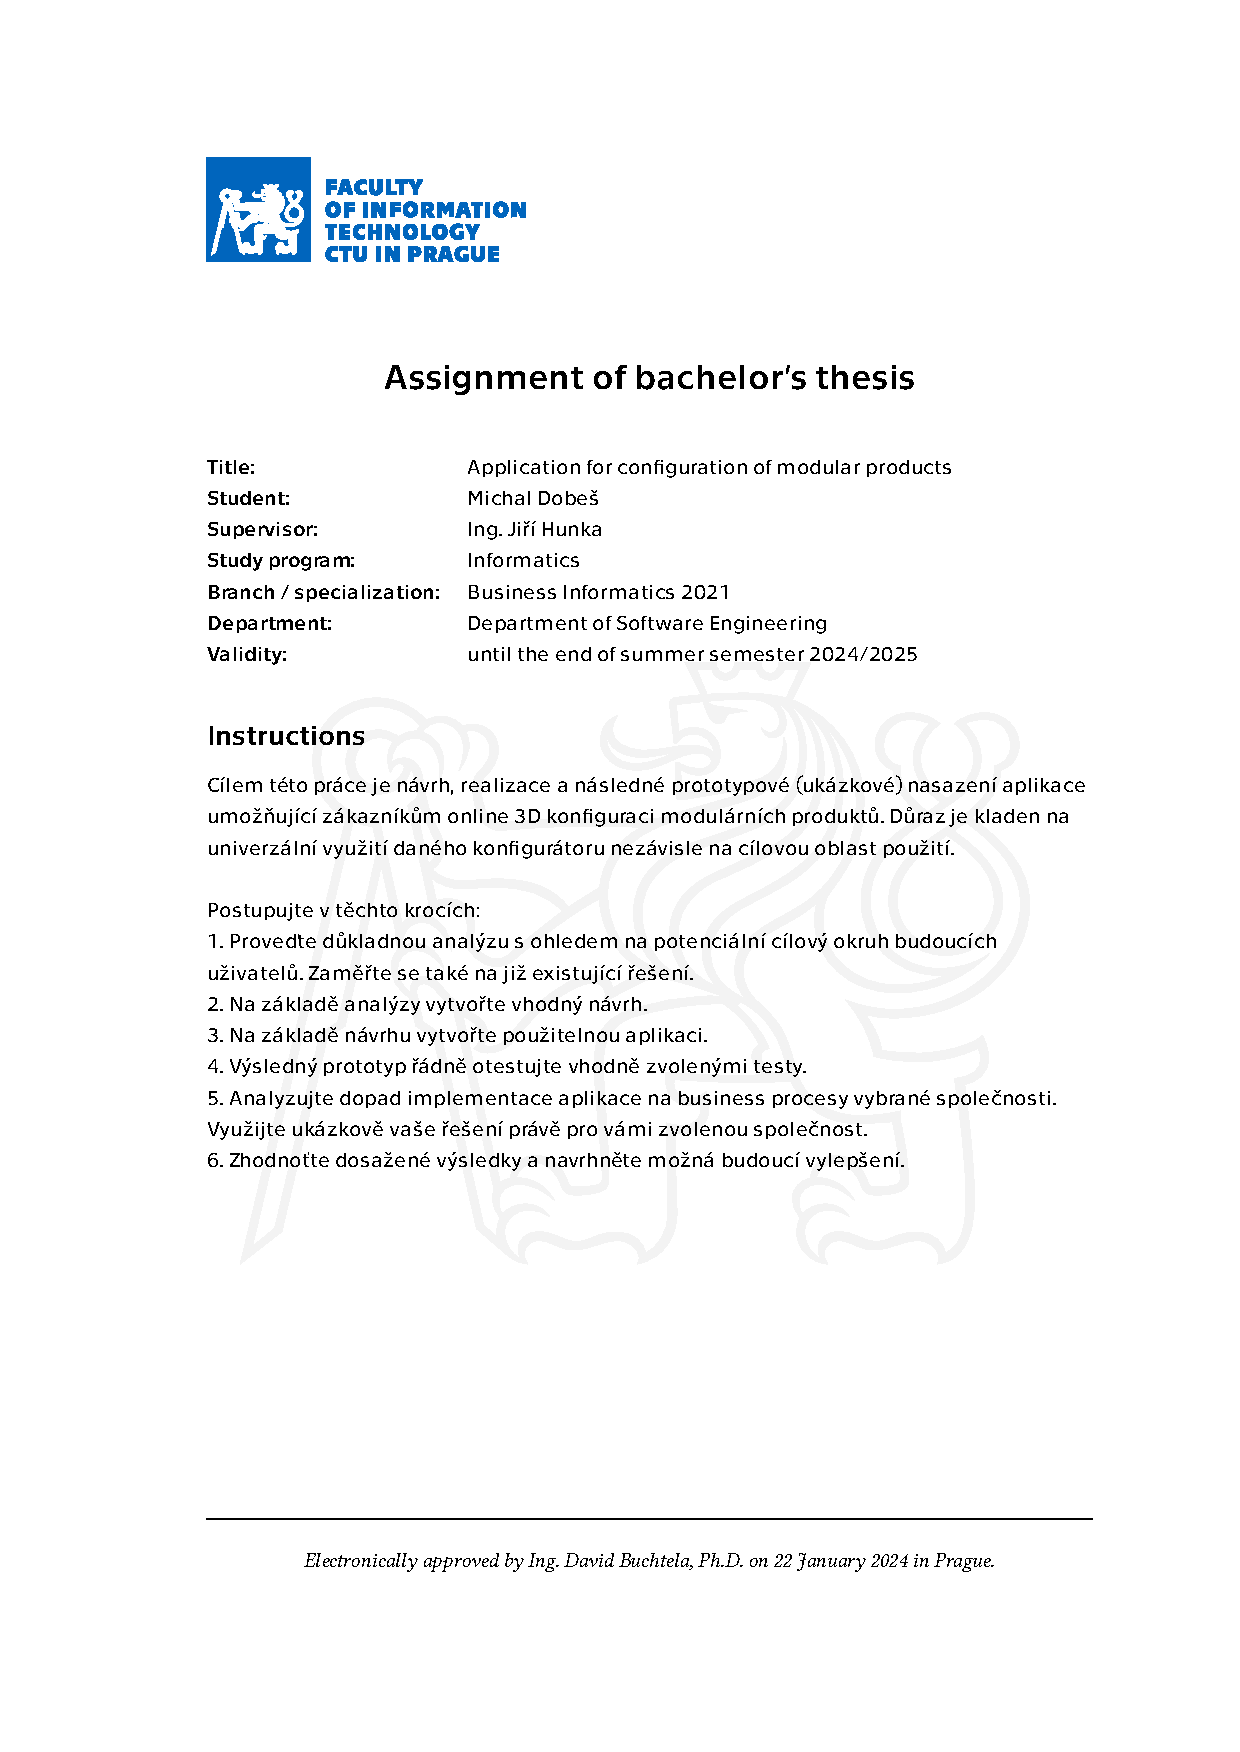
\includepdf[pages={1-}]{dobesmic-assignment.pdf} % replace that file with your thesis assignment provided by study office

\thispagestyle{empty}\cleardoublepage\maketitle % do not remove these three commands

\imprintpage % do not remove this command

\tableofcontents % do not remove this command
%%%%%%%%%%%%%%%%%%%%%%
% list of other contents: figures, tables, code listings, algorithms, etc.
% add/remove commands accordingly
%%%%%%%%%%%%%%%%%%%%%%
\listoffigures % list of figures
\begingroup
\let\clearpage\relax
\listoftables % list of tables
\lstlistoflistings % list of source code listings generated by the listings package
% \listoflistings % list of source code listings generated by the minted package
\endgroup
%%%%%%%%%%%%%%%%%%%%%%
% list of other contents END
%%%%%%%%%%%%%%%%%%%%%%

%%%%%%%%%%%%%%%%%%%
% ACKNOWLEDGMENT
% FILL IN / MODIFY
% This is a place to thank people for helping you. It is common to thank your supervisor.
%%%%%%%%%%%%%%%%%%%
\begin{acknowledgmentpage}
	I would like to thank...
\end{acknowledgmentpage} 
%%%%%%%%%%%%%%%%%%%
% ACKNOWLEDGMENT END
%%%%%%%%%%%%%%%%%%%


%%%%%%%%%%%%%%%%%%%
% DECLARATION
% FILL IN / MODIFY
%%%%%%%%%%%%%%%%%%%
% INSTRUCTIONS
% ENG: choose one of approved texts of the declaration. DO NOT CREATE YOUR OWN. Find the approved texts at https://courses.fit.cvut.cz/SFE/download/index.html#_documents (document Declaration for FT in English)
% CZE/SLO: Vyberte jedno z fakultou schvalenych prohlaseni. NEVKLADEJTE VLASTNI TEXT. Schvalena prohlaseni najdete zde: https://courses.fit.cvut.cz/SZZ/dokumenty/index.html#_dokumenty (prohlášení do ZP)
\begin{declarationpage}
FILL IN ACCORDING TO THE INSTRUCTIONS. VYPLNTE V SOULADU S POKYNY.
\end{declarationpage}
%%%%%%%%%%%%%%%%%%%
% DECLARATION END
%%%%%%%%%%%%%%%%%%%

\printabstractpage % do not remove this command

%%%%%%%%%%%%%%%%%%%
% SUMMARY
% FILL IN / MODIFY
% OR REMOVE ENTIRELY (upon agreement with your supervisor)
% (appropriate to remove in most theses)
%%%%%%%%%%%%%%%%%%%
% \begin{summarypage}
% \section*{Summary section}
% 
% \lipsum[1][1-8]
% 
% \section*{Summary section}
% 
% \lipsum[2][1-6]
% 
% \section*{Summary section}
% 
% \lipsum[3]
% 
% \section*{Summary section}
% 
% \lipsum[2]
% 
% \section*{Summary section}
% 
% \lipsum[1][1-8] Lorem lorem lorem.
% \end{summarypage}
%%%%%%%%%%%%%%%%%%%
% SUMMARY END
%%%%%%%%%%%%%%%%%%%

%%%%%%%%%%%%%%%%%%%
% ABBREVIATIONS
% FILL IN / MODIFY
% OR REMOVE ENTIRELY
% List the abbreviations in lexicography order.
%%%%%%%%%%%%%%%%%%%
\chapter{Abbreviations}
	
\begin{tabular}{rl}
AR & Augumented Reality\\
SPA & Single-Page Application\\
USDZ & Universal Scene Description Zip\\
API & Application Programming Interface\\
WebGL & Web Graphics Library\\
HTML & HyperText Markup Language\\
R3F & React Three Fiber\\
CSS & Cascading Style Sheets\\
\end{tabular}
%%%%%%%%%%%%%%%%%%%
% ABBREVIATIONS END
%%%%%%%%%%%%%%%%%%%

\mainmatter\mainmatterinit % do not remove these two commands

%%%%%%%%%%%%%%%%%%%
% THE THESIS
%%%%%%%%%%%%%%%%%%%

% \chapter{Introduction}
% uncomment the following line to create an unnumbered chapter
\chapter*{Introduction}\addcontentsline{toc}{chapter}{Introduction}\markboth{Introduction}{Introduction}
\setcounter{page}{1}

% The following environment can be used as a mini-introduction for a chapter. Use that anyway it pleases you (or comment it out). It can contain, for instance, a summary of the chapter. Or, there can be a quotation.
\begin{chapterabstract}
Product configurators and their value.
\end{chapterabstract}
\todo{Update headlines to title-case}
Over the past few decades, the rise of e-commerce has caused a shift in consumer expectations, resulting in an increased demand for individualized products. This gives rise to the need to shift focus towards mass customization, where products are customized according to individual preferences. To thrive in this sector, companies must modify their product offerings to meet the unique needs of users. This necessitates the existence of a system that enables customers to express their preferences and convert them into product configurations. \cite{Fulkerson2000}

The task of transforming user preferences into concrete designs is a difficult endeavor that can be hindered by a lack of effective communication between the customer's explanation of their desires and the business's comprehension. The use of online product configurators seemingly provides a solution to this issue by offering a user-friendly and visually appealing platform that allows customers to customize products according to their specifications, improves the customer experience by increasing engagement and interactivity, and helps bridge the gap between customer expectations and the end product. These tools have become an integral part of successful personalization strategies. \cite{Franke2003}

The involvement of consumers in the customization process leads to a stronger bond with the product, resulting in a perception of a higher value of the product compared to standard off-the-shelf products. This aspect of mass customization makes it an appealing and compelling strategy for businesses to implement. \cite{Schreier2006} However, when implementing such a system, it is crucial to ensure that the customization process is pleasurable for the customer. Research has shown that the enjoyment experienced during the customization process also affects the perceived value of the final product, highlighting the importance of good implementation. \cite{Franke2010}

The introduction of modern technologies such as WebGL or Augmented Reality (AR) has expanded the potential of online configurators. These advances enable these toolkits to become more powerful and visually illustrative tools that provide a higher level of interactivity and realism than what was previously accessible. \cite{Cozzi2015}

%---------------------------------------------------------------
\section{Objective of this thesis}
%---------------------------------------------------------------

The primary objective of this thesis is to design and implement an application (toolkit) for the online configuration of modular products. The toolkit aims to be product-agnostic, adaptable, and customizable, usable by various businesses, enabling their customers to customize their modular products interactively. The focus is on ensuring that the toolkit is not only flexible in accommodating various specific needs, but also straightforward for businesses to maintain after deployment, emphasizing lightweight infrastructure requirements. 

To accomplish this main objective, an accompanying analysis of the characteristics found in current product configurators is required, as well as an examination of comparable solutions currently available to businesses.

%---------------------------------------------------------------
\section{Structure of this thesis}
%---------------------------------------------------------------

This thesis is divided into six chapters.

\begin{description}
\item[Chapter 1] The initial chapter entails an examination of existing solutions and an investigation into the functionalities that should be incorporated into this particular application.

\item[Chapter 2] The second chapter discusses the design of the application, the technologies chosen, the architecture, and the data structures.

\item[Chapter 3] The third chapter is devoted to implementation.

\item[Chapter 4] Chapter four focuses on the deployment of the implemented application in a particular business as an example. In addition, it discusses the resulting changes in the business processes of a chosen example business.

\item[Chapter 5] In the fifth chapter, the tests used in the development of the application are described.

\item[Chapter 6] Finally, the last chapter summarizes the results achieved and suggests possible directions for future development.
\end{description}
\chapter{Analysis}

\begin{chapterabstract}
A comprehensive evaluation of existing solutions, identification of key features and limitations, and outlining of the specifications for the proposed solution.
\end{chapterabstract}

Product configurators can be implemented in various ways, and the design of the tool itself determines the types of products that can be customized using the tool later on. The number of unique configurations of a product that the tool can create is called the solution space. The size of the solution space is determined by the count of customizable attributes and the achievable values of each attribute.~\cite{Huiwen2018} A relevant study examined the solution spaces of these toolkits and proposed an evaluation model that enables the categorization and assessment of various implementation approaches. Based on the target outcome and the guidance provided by the tool, the following mechanisms are defined:~\cite{Hermans2012}

\begin{definition}[Veneer]
Customization by adding a visual decorative layer. (e.g., printing, engraving, etching)
\end{definition}
\begin{definition}[Modularity]
Customization by combining modules or components.
\end{definition}
\begin{definition}[Parametric]
Customization by changing the parameter values of parts.
\end{definition}
\begin{definition}[Generative]
Customization using code and scripting to synthesize the final form of the product.
\end{definition}

There are often some common characteristics among configuration tools with different mechanisms; however, the main focus of this thesis is on toolkits that primarily employ modularity mechanisms.
\newpage

%---------------------------------------------------------------
\section{Existing Solutions}
%---------------------------------------------------------------
% - - - - - - - - - - - - - - - - - - - - - - - - - - - - - - -
\subsection{Applications of Product Configurators}
% - - - - - - - - - - - - - - - - - - - - - - - - - - - - - - -

Many companies across multiple industries, such as automotive, fashion, furniture, housing, are integrating product configurators into their sales strategies. These configurators serve as the main or supplementary sales tools for these businesses.

The Configurator Database Project by cyLEDGE MEDIA aims to catalog these web-based configuration tools. The 2017/2018 report tracked 1250 deployments of these tools; however, the true count will be significantly higher since the database only includes the most frequently visited applications.~\cite{cyLEDGE2018}

An analysis of the 100 most viewed configurators from May 2020 to May 2021 in the Configurator Database Project was performed in a study that examined the shared characteristics of these configurators.~\cite{Blazek2023} The summary of some of the relevant characteristics and design choices that the study has analyzed are presented in this section:
\begin{description}
    \item[Responsive design:] 75.3\% of examined tools had responsive design (the design adapted to the viewport of the device).
    \item[Navigation:] 17.5\% of configurators had linear predefined navigation (meaning the configuration had to follow a specified sequence), whereas the 82.5\% majority of tools had open navigation (meaning the user has the flexibility to configure the product in any order).
    \item[Visualization:] 79.4\% of tools utilized photorealistic visualization (as opposed to illustrations or no visualization); however, the study acknowledges that there were significant variations depending on the industries in which the configurator is utilized.
    \item[Data transfer:] The mean network data size transferred for 3D configurator was 35.6~MB.
    \item[Configuration options:] 60.8\% of configurators offered more than ten customizable attributes.
    \item[Purchase capability:] Given that car brands typically do not directly sell their cars online, they were excluded from the analysis of this particular characteristic. Without vehicle configurators, 70.5\% of the configurators could complete an online purchase of the configured product.
    \item[Price calculation:] 56.7\% of the configurators were able to instantly reflect the changes made to the configuration in the displayed price.
\end{description}

The previous paragraphs discussed general trends among all product configurators of all kinds. As part of the analysis in this chapter, it is essential also to examine existing modular 3D product configurators. 

Due to the large number of existing applications, it is not within the scope of this work to perform an exhaustive analysis. Instead, this section will focus on a select group of three applications. These have been selected based on a combination of factors such as their popularity, functionality, and importance in the context of a modular product configuration. This selection is intended to provide insightful examples that highlight different approaches, rather than being representative of the entire domain.

\noindent The main aspects under consideration are as follows:\nopagebreak
\begin{itemize}[label=\rectanglebullet]
    \item \textbf{Platform:} How is the application accessible?
    \item \textbf{Navigation:} How does the user navigate in the application during the configuration process?
    \item \textbf{Visualization style:} How is the product visualized within the configuration process?
    \item \textbf{Placement options:} Can the modular components be freely placed, or are they restricted to fixed points?
    \item \textbf{Camera movement:} From which angles can the product be visualized, and how can it switch between them? In the context of the tool, camera refers to a virtual camera in a 3D graphical environment that simulates the viewpoint and perspective from which the 3D scene is viewed.
    \item \textbf{Impossible configurations:} Is it possible to create configurations that are not feasible in reality?
    \item \textbf{Responsiveness:} How does the application adapt to different device viewports?
    \item \textbf{Price calculation:} Is the price of the configured product calculated in real-time?
    \item \textbf{Purchase option:} Is there an option to finalize and purchase the configured product within the application?
    \item \textbf{Save option:} Can users save their configurations to return to them later?
    \item \textbf{Version history:} Does the configurator provide an accessible history of configuration changes?
    \item \textbf{\noborderacrshort{vr} or \noborderacrshort{ar}:} Can the configured product be visualized in \noborderacrlong{vr} or \noborderacrlong{ar}?
    \item \textbf{Real dimensions}: Can the configurator display information about the real dimensions of the configured products? 
\end{itemize}
\break
\noindent Furthermore, the design decisions are also discussed:\nopagebreak
\begin{itemize}[label=\rectanglebullet]
    \item \textbf{Views:} What is the position and size of the views inside the application?
    \item \textbf{Navigation bars:} Where are the navigation bars placed and how are they utilized?
    \item \textbf{Button placements:} How are different buttons placed within the application's interface?
\end{itemize}


%______________________________________________________________
\subsubsection{IKEA PAX Planner}

IKEA is a widely recognized global home furnishings retailer specializing in affordable furniture.~\cite{StatistaIkea}

IKEA offers the PAX fitted wardrobe, for which they not only sell predefined configurations, but also allow customers to modularly choose the ideal size, doors, knobs, handles, interior organization, and lightning.~\cite{IkeaPAX}

To accomplish this, they utilize the PAX Planner web tool.\footnote{Available at: \url{https://www.ikea.com/addon-app/storageone/pax/web/latest/cz/en/}}

\begin{figure}[h]
\centering
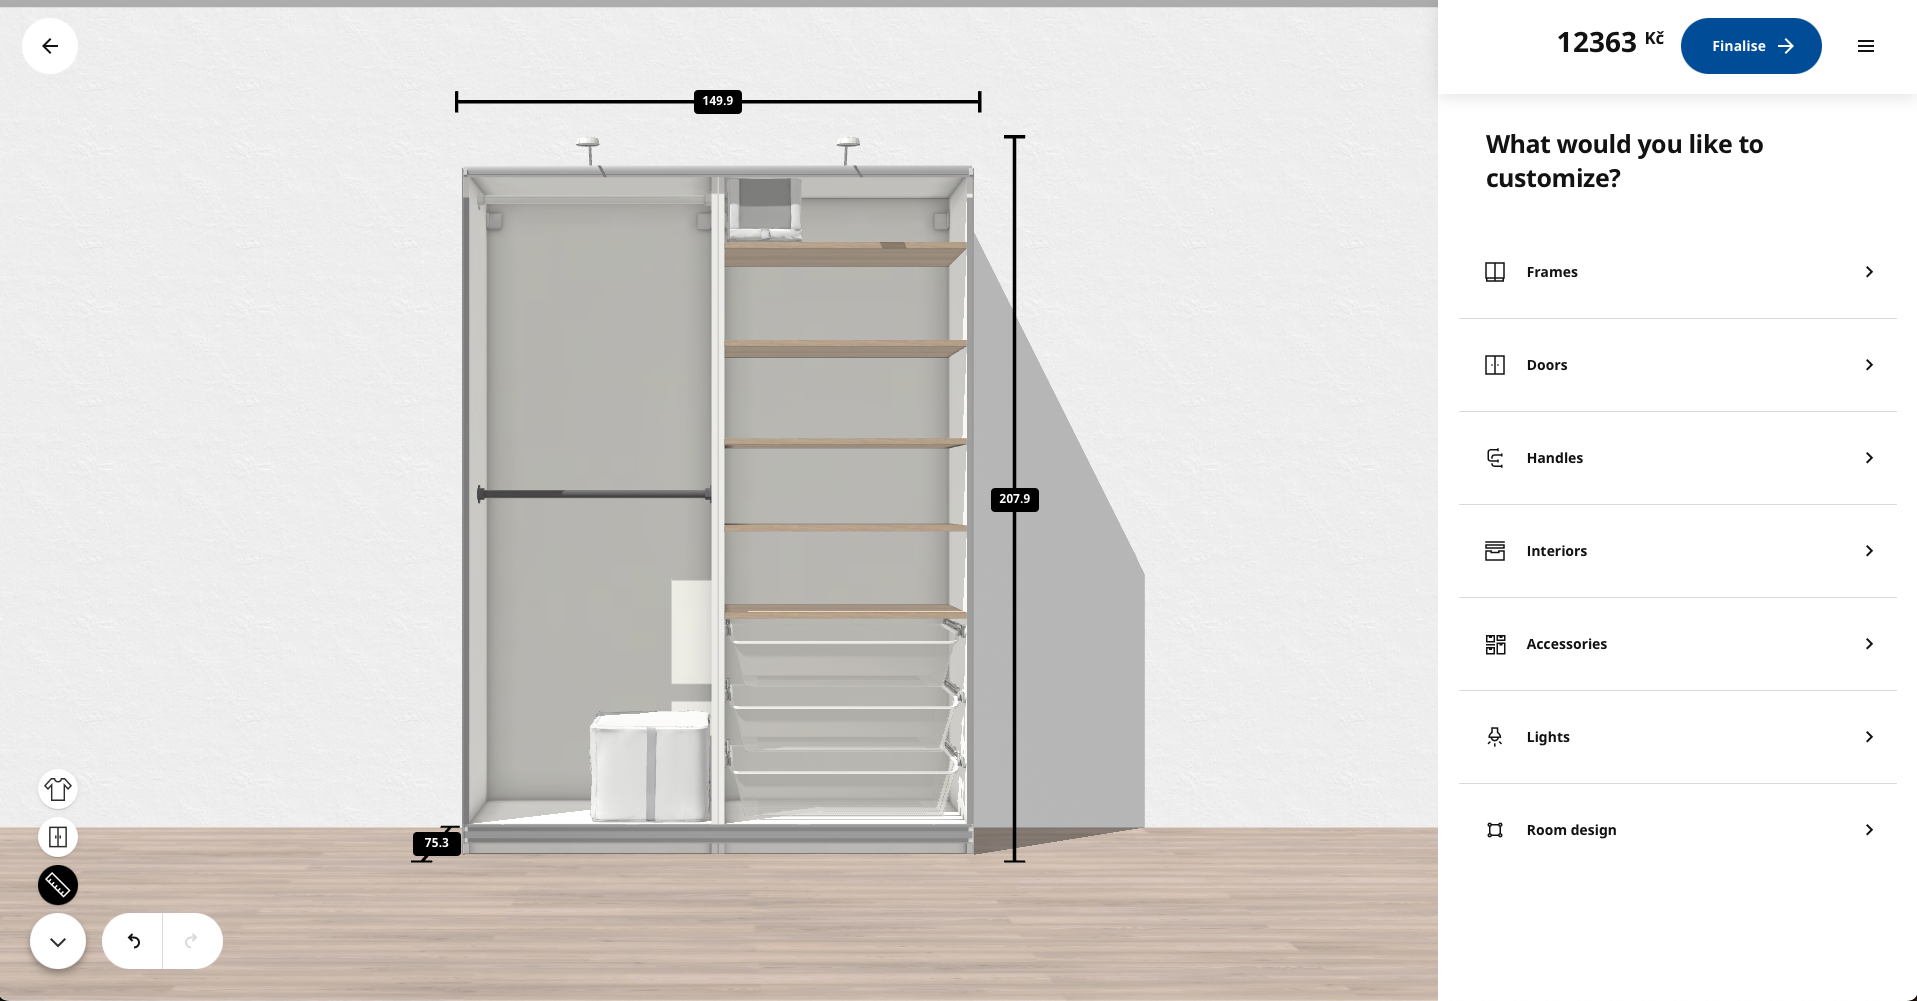
\includegraphics[width=\textwidth]{images/analysis_ikea-pax.png}
\captionsource{Screenshot of IKEA PAX Planner Tool with example configuration}{IKEA~\cite{IkeaPAX}}
\end{figure}

The tool consists mainly of two views. The primary view on the left contains a 3D preview of the configured product, allowing users to observe objects from different viewpoints by moving along an orbital trajectory in a 180-degree half-circle. The components displayed in the 3D view are both realistic and interactive. Users can adjust their position by dragging, and selecting a component offers additional information along with real-life images of the item. All modular options that can be added to the current configuration are found in the secondary smaller view on the right side and can be added by clicking or dragging them into the 3D preview. The application is responsive, and on mobile devices, the secondary view moves from the right side to a bottom sliding panel. The navigation bar is located at the top of the secondary view, and other buttons are located around the edges of the primary view.

At the beginning of the configuration process, the application prompts the user to select the starting point of the configuration. The configurator has open navigation, meaning that the components can then be configured in any order. Components can be placed anywhere along a specified axis with certain restrictions, effectively preventing the creation of impossible configurations.

The tool performs live price calculations and contains a final summary confirmation screen from which it is possible to order the configured product in the e-shop. The configurator maintains a history of recent changes, accessible through undo and redo buttons. It also features the ability to save configurations on the server, which can be retrieved later using a generated code.

The configurator also provides a range of innovative features, such as the ability to change the visibility of some elements using a button (e.g. hiding the doors of a wardrobe to reveal the contents inside) or the ability to display dimensions directly in the 3D preview.

The application is a \noborderacrfull{spa} and does not update the \noborderacrshort{url} based on the selected product or phase of the configuration.

\noborderacrshort{spa} is a web application implementation approach that loads only a single page and then sequentially updates the content of the page with scripting on the client side, rather than loading whole new pages from the server.~\cite{Fink2014}


%______________________________________________________________
\subsubsection{Muuto Product Planner}

Muuto is a Scandinavian design company that produces furniture and home accessories. \cite{Muuto}

The company provides Product Planner, a 3D web-based configurator, which allows customers to customize and combine the designs of various products, such as storage systems, sofas, tables, or wall hangers, tailored to their specific needs.\footnote{Available at: \url{https://planner.muuto.com/}}~\cite{MuutoPlanner}

\begin{figure}[h]
\centering
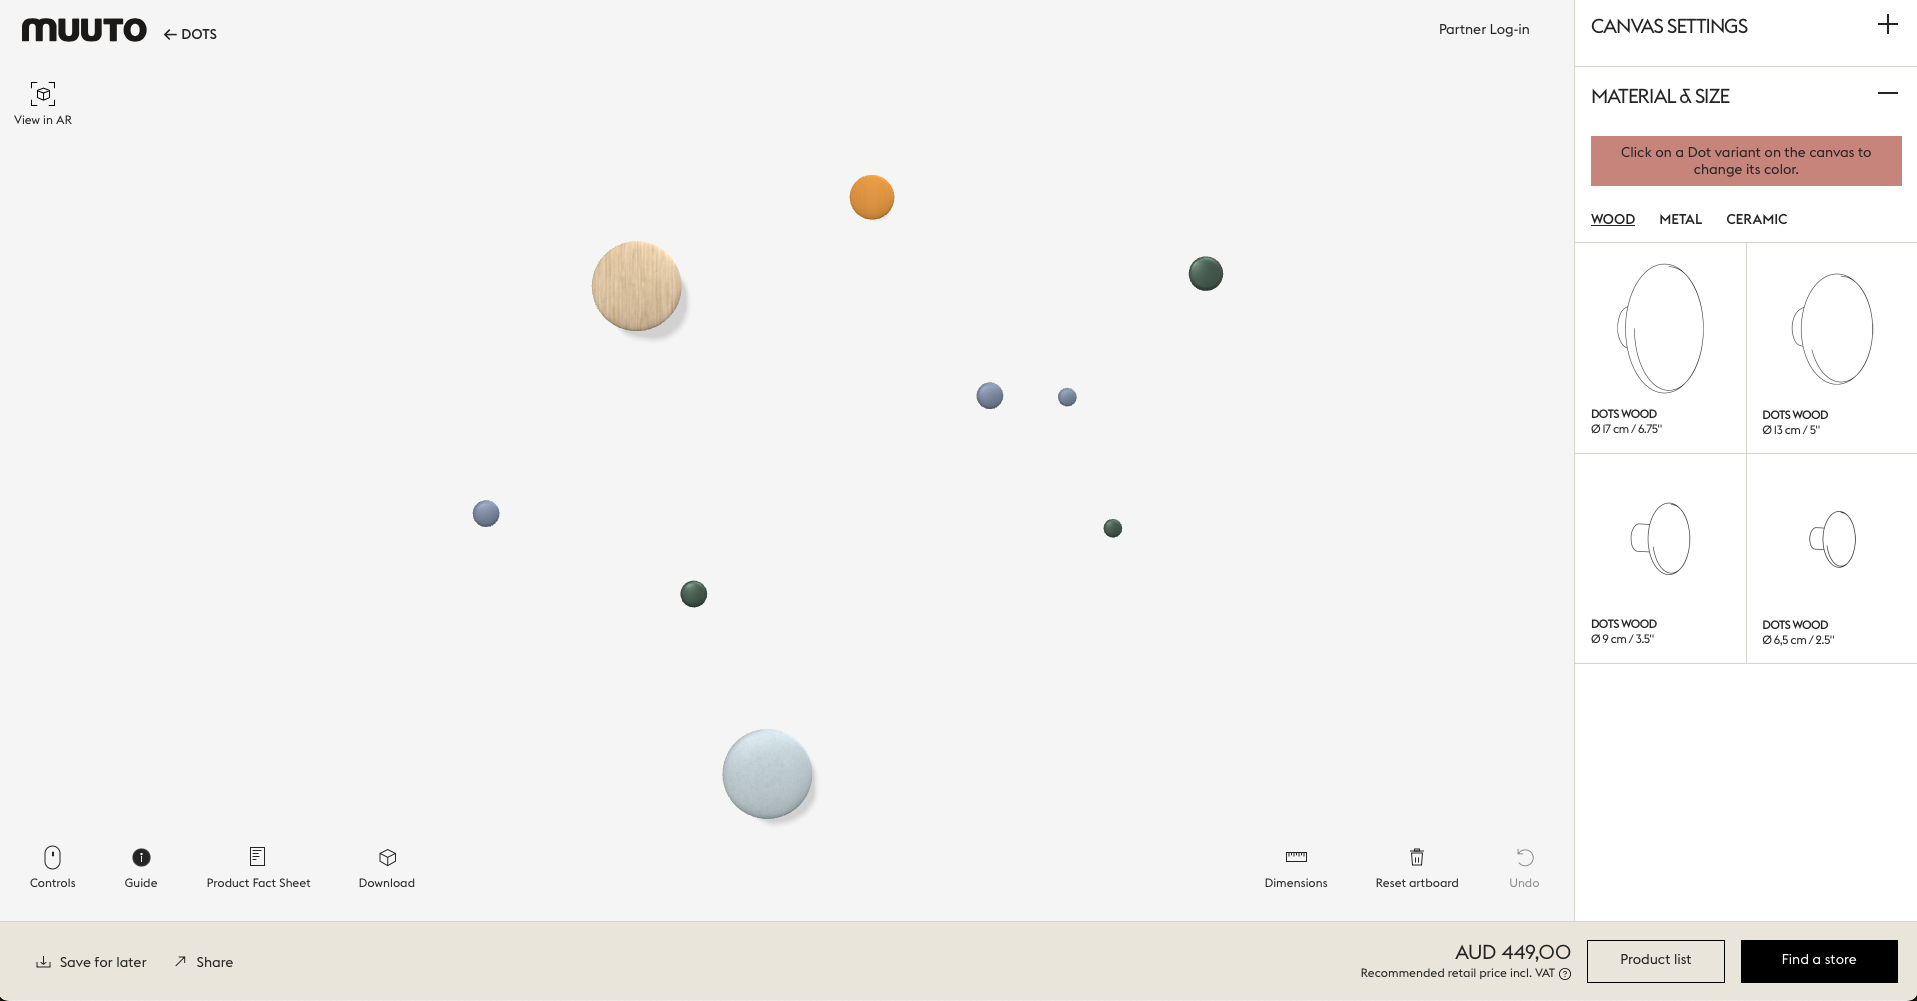
\includegraphics[width=\textwidth]{images/analysis_muuto-product-planner.png}
\captionsource{Screenshot of Muuto Product Planner tool with example configuration}{Muuto~\cite{MuutoPlanner}}
\end{figure}

The design of the configurator is similar to that in the previous case. The configurator also consists of two views. The primary view on the left provides full realistic 3D visualization, while the smaller secondary view on the right side allows users to add components by dragging them into the main view. Selecting a component in the primary view enables users to remove it or alter its materials. As the design is responsive, on smaller devices, the secondary view transforms into a bottom slide panel. Depending on the configured product, the tool offers a preview either from a single angle or a preview from any point on an orbital trajectory. The main view is also surrounded by buttons along its edges. The navigation bar is positioned at the bottom across the entire application, while the company logo is displayed on the top left.

The tool follows a similar flow, starting with the selection of the starting point and then moving to the configurator process, which has open navigation. Components can be placed anywhere, unless their position is dependent on another component. Due to this flexibility and also the wide variety of products that it supports, the configurator is not restricted to generating configurations that are feasible to produce and can create impossible configurations.

The tool can display real dimensions and can reverse the performed changes using the undo and redo buttons. The configuration can also be saved on the server-side and later accessed using a unique code. Live price calculation is also performed, and there is a summary page, but it is not possible to order the configured product; instead, the user is redirected to a physical store locator.

Furthermore, the designed configuration can be quickly shared with other users using email, or it can be downloaded in several file formats containing the 3D model itself. The application makes it possible to view the product in \noborderacrshort{ar}, directly in a web browser, albeit only on Apple devices using the \noborderacrfull{usdz} format and \noborderacrshort{ar}~Quick Look.~\cite{Jackson2018}

The application has multiple URL schemes that depend on the configuration phase, but they are not determined by the current product. 

%______________________________________________________________
\subsubsection{LD Seating Nido Configurator}

LD Seating is a company based in the Czech Republic that specializes in the production of chairs, armchairs, and sofas.~\cite{LDSeating}

The company uses a 3D web-based configurator to market the Nido modular seating system, which consists of elements that are designed to be combined in various ways.\footnote{Available at: \url{https://nido.ldseating.com/en/configurator}}~\cite{NidoConfigurator}

\begin{figure}[ht]
\centering
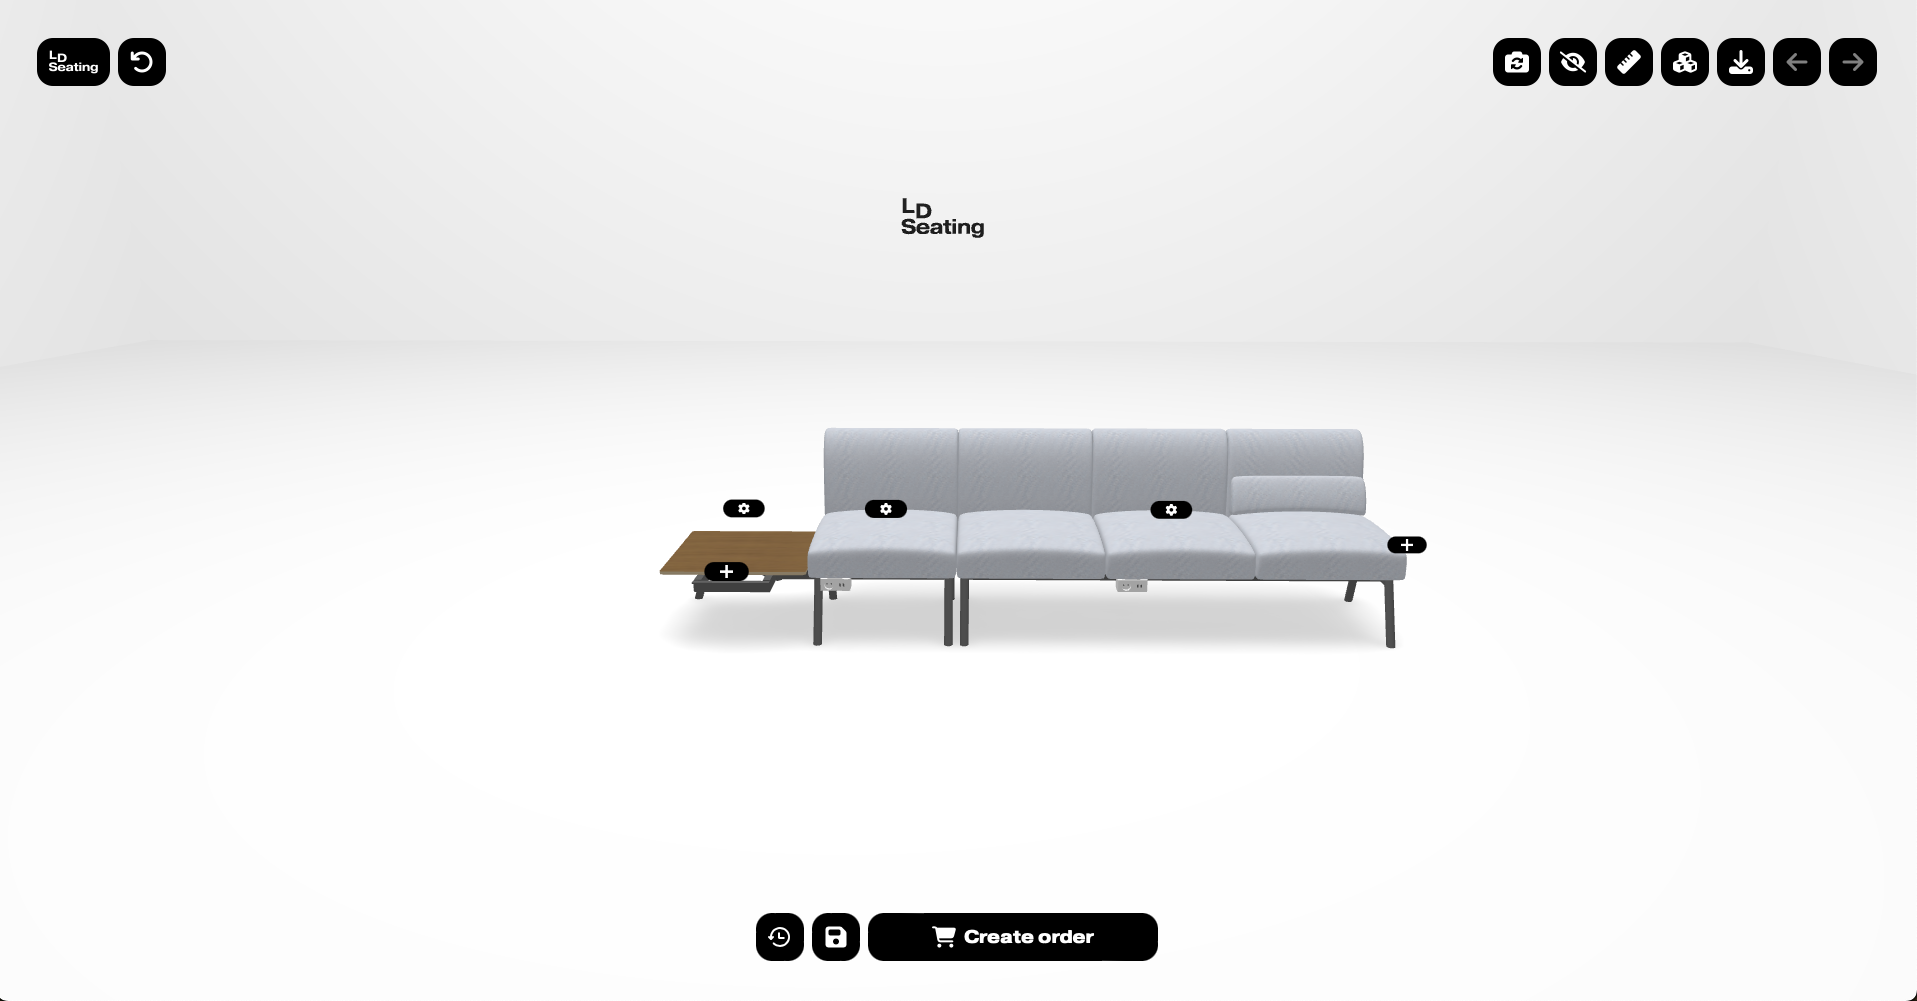
\includegraphics[width=\textwidth]{images/analysis_nido-configurator.png}
\captionsource{Screenshot of LD Seating Nido Configurator with example configuration}{LD Seating~\cite{NidoConfigurator}}
\end{figure}

The configurator consists of one large view, covering the whole application, which displays high-definition 3D models of the configured components. The buttons are placed around the entire view, on the top right, bottom center, and top left, where the company logo is also displayed.  The controls for adding components and modifying properties are embedded directly in the 3D scene. When necessary, a panel opens to the right, allowing users to select components to add, adjust component properties, or change materials. The application is partially responsive, as the side panel opens fullscreen on smaller viewports; however, there are some issues with image and text overflows on mobile devices. The main view allows the user to observe the configuration from all angles along an orbital trajectory.

The flow of the application also includes selecting a starting point. The product configuration process itself uses open navigation. The tool assesses whether a component can fit into a space and, if not, prevents its placement, thereby restricting impossible configurations. At the completion of the configuration, a confirmation summary is presented; however, in this case, the price is not calculated live. The configurator cannot directly place an order for the product, but instead confirming results in the display of an inquiry form.

The resulting configuration can be downloaded as a file containing the 3D models. The configuration can also be saved server-side, which generates a unique link at which the configuration is accessible. The tool features a version history that stores each saved configuration for future access. Users can revisit these versions, while undo and redo buttons are also available. The resulting configuration can also be exported to a \noborderacrshort{pdf} file containing a list of components. The tool also has the ability to display real dimensions.

The application is a \noborderacrshort{spa}, maintaining a consistent \noborderacrshort{url} and changing it to reflect the location of a saved configuration (if one exists).


% - - - - - - - - - - - - - - - - - - - - - - - - - - - - - - -
\subsection{Available Toolkits}
% - - - - - - - - - - - - - - - - - - - - - - - - - - - - - - -

In this section of the analysis chapter, the focus shifts from specific 3D modular configurator applications to the fundamental toolkits that power the configurators. Although many configurators are bespoke and tailored to the specific needs of companies and their individual products, there are providers offering more generic and adaptable solutions. These offerings are highly relevant to this thesis, as the objective of this thesis is to create a product-agnostic toolkit, which means that there is a need to consider the way the configurator is set up by the business.

A variety of providers offer these toolkits for deploying product configurators, intending to provide semi-custom or fully custom solutions, as well as generic options. This section examines two particular toolkits to carry out a focused and relevant analysis. The choice of toolkits analyzed has been complicated by the fact that most providers are cautious about the details of the technology, typically revealing in-depth information only after a serious business inquiry. The choice was also based on factors such as the implementation approach and compatibility with modular products.

\noindent This section seeks to answer the following questions about the toolkits: 
\begin{itemize}[label=\rectanglebullet]
    \item \textbf{Administration}: How is the product configurator created and administered?
    \item \textbf{Assets}: How are assets stored and cataloged?
    \item \textbf{Product configuration}: How are the configuration options and rules defined?
    \item \textbf{Integration}: How is the tool integrated into other systems?
    \item \textbf{Pricing}: What is the cost of the offered solution?
\end{itemize}


%______________________________________________________________
\subsubsection{Threekit}

Threekit is a leading global company in visual commerce technologies that specializes in 3D product visualizations. The Threekit Platform, which enables clients to create interactive product experiences according to their needs, functions as an administrative application and has the capability to generate product configurators (see \autoref{fig:threekit-platform} in \autoref{appendix-a}).~\cite{ThreeKitAboutUs, ThreeKitPlatform}

The platform is very complex with many distinct features. At its core, it uses a catalog for storing all product data (the products themselves, materials used, configurable parts, etc.). The items in the catalog can then be loaded into The Treekit Player, which will display the models in 3D, with the option for users to change attributes (models and materials) that are tied to the item. The behavior of the configurator can be set up using item rules and logic that support conditions, queries, and even custom scripts. The platform also offers a data tables feature that is similar to spreadsheets and is designed to handle extensive configuration data and logic. The application also has a built-in asset editor for refining 2D and 3D assets and configuration options (see \autoref{fig:threekit-editor} in \autoref{appendix-a}). Models of the products can be uploaded in various 3D formats. The platform provides \noborderacrshort{api} integration with the leading e-commerce and \noborderacrshort{erp} systems.~\cite{ThreeKitPlatformDocumentation}

The offered solution is still partially tailored to the client, which is the reason why the service does not have standardized pricing. Instead, the price is determined through a personalized quote. It is important to note that the analysis of Threekit presented here is based on the publicly available documentation of the platform. Direct access to the full suite of Threekit's tools is typically available only after formalizing a business agreement with the company.


%______________________________________________________________
\subsubsection{Roomle}

Roomle is an Austrian company focused on pioneering visual product configuration. They provide solutions for product visualization, room design, and product configurators. Roomle's solution, called Rubens, is described as a \enquote{Open Full Logic 3D-Configurator}. The tool utilizes both parametric and modular configuration mechanisms. The software allows integration with third parties through the use of an \noborderacrshort{api}. In addition, it supports integration with other front-end technologies on web and mobile platforms and has a built-in \noborderacrshort{ar} experience.~\cite{RoomleAbout}

A web application, Rubens Admin, is used to set up the configurator application. To add a product that can then be configured by customers, 3D models, and materials are uploaded to the admin application. Components are defined using RoomleScript language, which is loosely based on the JavaScript language. The design of the configurator itself can be tuned in the admin application as well. Multiple language variants can be defined for product names and descriptions. The configurator application (see \autoref{fig:roomle} in \autoref{appendix-a}) runs on the client-side and can be simply embedded into a website. Additionally, a JavaScript library that can subscribe to events or modify the configurator can be utilized. A framework is also provided to utilize the configurator within an iOS application.~\cite{RoomleDocumentation}

In terms of pricing, Roomle's Rubens configurator with the listed capabilities is offered to businesses at a monthly fee of €1450.~\cite{RoomleFullLogic}

% - - - - - - - - - - - - - - - - - - - - - - - - - - - - - - -
\subsection{Summary of Existing Solutions}
% - - - - - - - - - - - - - - - - - - - - - - - - - - - - - - -

\begin{table}[htb!]
\centering
\begin{tabular}{>{\raggedright\arraybackslash}p{3.8cm}*{3}{>{\centering\arraybackslash}p{2.5cm}}} 
\toprule
\parbox[c][7ex]{3.8cm}{\textbf{Features}} &
\multrow{c}{\textbf{IKEA} \\ \textbf{Pax} \\ \textbf{Planner}} &
\multrow{c}{\textbf{Muuto} \\ \textbf{Product} \\ \textbf{Planner}} &\multrow{c}{\textbf{LD Seating} \\ \textbf{Nido} \\ \textbf{Configurator}} \\ 
\midrule
\parbox[c][7ex]{3.8cm}{Platform}
    & Web
    & Web
    & Web \\ 
\parbox[c][7ex]{3.8cm}{Navigation}
    & Open
    & Open
    & Open \\ 
\parbox[c][7ex]{3.8cm}{Visualization}
    & Realistic
    & Realistic
    & Realistic \\ 
\parbox[c][7ex]{3.8cm}{Placement options}
    & Free
    & Free
    & Fixed points\\ 
\parbox[c][7ex]{3.8cm}{Camera movement}
    & Orbital
    & \multrow{c}{Orbital; \\ Static}
    & Orbital \\
\parbox[c][7ex]{3.8cm}{Impossible \\ configurations} 
    & No
    & Yes
    & No \\
\parbox[c][7ex]{3.8cm}{Responsiveness}
    & Yes
    & Yes
    & Yes \\
\parbox[c][7ex]{3.8cm}{Price calculation}
    & Yes
    & Yes
    & No \\
\parbox[c][7ex]{3.8cm}{Purchase option}
    & E-shop order
    & Store locator
    & Inquiry form \\
\parbox[c][7ex]{3.8cm}{Save option}
    & Server-side
    & \multrow{c}{Server-side; \\ Local}
    & \multrow{c}{Server-side; \\ Local} \\
\parbox[c][7ex]{3.8cm}{Version history}
    & Undo \& redo 
    & Undo \& redo
    & \multrow{c}{Undo \& redo; \\ Multiple saves} \\
\parbox[c][7ex]{3.8cm}{VR or AR}
    & No
    & Yes
    & No \\
\parbox[c][7ex]{3.8cm}{Real dimensions}
    & Yes
    & Yes
    & Yes \\
\bottomrule
\end{tabular}
\caption{Summary of key points discussed in the analysis of existing modular product configurators}
\label{table:summary-analysis}
\end{table}

All the product configurators analyzed have common characteristics, especially in terms of navigation and visualization styles, which remain consistent across different tools. Despite this, certain trade-offs were observed between them, especially regarding placement options. While some solutions offer users the freedom to position components anywhere, others restricted placement to fixed points. This variance stems from implementation complexity, as the fixed-point system is simpler, furthermore offering a better way to restrict impossible configurations.
Another significant distinction was observed in the product finalization process, which ranged from the ability to place an order to being directed to a physical store.

The key points discussed in the analysis of modular product configurators are summarized in \autoref{table:summary-analysis}.

The user interface design of the analyzed configurations also displayed similarities, particularly in layout style, featuring a primary 3D preview on the left, a secondary view on the right, and buttons surrounding the primary view.

Analyzing the offered toolkit solutions proved challenging due to the information being closely guarded, as it is in the financial interest of the providers. However, the examined toolkits are very sophisticated solutions that are supported by large backend services, which are used for storing assets and facilitating the configurators functionality. The toolkits offer advanced features that allow for the definition of rules and logic, allowing companies to create configurators with a large amount of complexity. This indicates that these toolkits target a market composed mainly of larger corporations that require sophisticated solutions, which is also reflected in pricing.

%---------------------------------------------------------------
\section{Proposed Solution}
%---------------------------------------------------------------

This thesis aims to develop a new solution for the configuration of modular products. To do so, the proposed solution will incorporate the common characteristics identified in the analyzed solutions. The following paragraphs of this chapter should answer the important questions of who, what, why and how, detailing the key aspects of the proposed solution. 

The main differentiation factor of this proposed toolkit is its emphasis on catering to small businesses. As the existing toolkits that were examined were costly and mainly aimed at larger companies, this solution aims to fill this market gap. To achieve this, it will be necessary to make some trade-offs ensuring the solution's adaptability and relevance across various product types without making the solution overly complex. Therefore, the proposed toolkit will prioritize simplicity and cost-effectiveness, following the best practices seen in larger-scale solutions but with a specific focus on the needs and capabilities of the target market.

The following chapter outlines the features that should be implemented in the solution proposed in this thesis.
 
The proposed toolkit is envisioned to be universal with regard to products, adaptable, and customizable, catering to a wide variety of modular products and industries. The solution should be simple for businesses to deploy and manage, without the need for extensive technical resources, ensuring that it is straightforward for smaller businesses to maintain and operate effectively.

% - - - - - - - - - - - - - - - - - - - - - - - - - - - - - - -
\subsection{Requirement Engineering} \label{section:requirements}
% - - - - - - - - - - - - - - - - - - - - - - - - - - - - - - -

Following the overview of objectives and the definition of the target market, it is necessary to formulate precise requirements for this solution. Detailing these features and characteristics is crucial for successful implementation. Thus, the description of requirement engineering for this solution will be provided here.

The process of requirement engineering for software products involves gathering, analyzing, selecting, and managing requirements. It focuses on interpreting and understanding the goals, needs, and beliefs of stakeholders and transforming them into specific requirements.~\cite{Aurum2005}

There are many ways to categorize software requirements, such as audience-oriented categorization or using the FURPS method, which classifies requirements based on functionality, usability, reliability, performance, or supportability.~\cite{Stephens2023}

Given that the majority of requirements for the solution fall either into the functionality or usability category, the requirements in this section are separated only into the following two main categories:~\cite{Aurum2005}
\begin{enumerate}
    \item Functional requirements: These requirements describe what the system should be able to do. They specifically outline the system's behavior and its interactions in specific situations.
    \item Non-functional requirements: These requirements put constraints on the solution that meets the functional requirements, rather than being focused on specific behaviors of the system. They are often, among others, focused on performance, security, accessibility, and compatibility.
\end{enumerate}

To manage and prioritize these requirements, each is assigned an approximate priority level using the MoSCoW method. This approach classifies the requirements into four distinct categories:~\cite{Stephens2023}
\begin{enumerate}
    \item Must: Requirements crucial for the final solution.
    \item Should: Requirements to be implemented if feasible.
    \item Could: Requirements that are desirable but not essential.
    \item Won't: Nice-to-have requirements that most likely will not be implemented in this solution.
\end{enumerate}
This method helps to plan and allocate resources throughout the implementation phase.

\break
Additionally, each requirement is given a rough estimate of the implementation difficulty, separated into three categories: \nopagebreak
\begin{enumerate}
    \item Simple: Requirements that are straightforward to implement and require little time and few resources.
    \item Intermediate: Requirements that pose moderate challenges and demand a considerable amount of resources, time, and problem-solving.
    \item Complex: Requirements that are highly challenging and involve substantial resources, time, and expertise.
\end{enumerate}
This preliminary assessment aims to classify the requirements without relying on specific rigid criteria for each category. This method is specifically used only for functional requirements, as non-functional requirements affect the software's functionality and user experience through abstract constraints, making them unsuitable for the same difficulty estimation approach.
% - - - - - - - - - - - - - - - - - - - - - - - - - - - - - - -
\subsubsection{Functional Requirements}
% - - - - - - - - - - - - - - - - - - - - - - - - - - - - - - -

\begin{enumerate}[label=\textbf{F\arabic*:}, leftmargin=*]
\item \label{itm:F1} 3D product visualization
\vspace{2pt}
\\The tool shall offer users 3D visualization of their configured product, employing realistic models to accurately represent the components used and their characteristics.
\begin{itemize}[noitemsep, label=\trianglebullet]
    \item \textbf{Priority:} Must
    \item \textbf{Difficulty:} Complex
\end{itemize}
\vspace{4pt}

\item \label{itm:F2} Dynamic orbital camera controls
\vspace{2pt}
\\The tool should have dynamic orbital camera controls that allow users to view the product in the 3D product visualization (see requirement \hyperref[itm:F1]{F1}) from any angle by rotating, panning, and zooming the camera around the product. This feature aims to provide an engaging visual experience that allows users to examine the product with a 360-degree view. The controls should be intuitive, allowing for seamless navigation through mouse actions or touch gestures depending on the device used.
\begin{itemize}[noitemsep, label=\trianglebullet]
    \item \textbf{Priority:} Must
    \item \textbf{Difficulty:} Simple
\end{itemize}
\vspace{4pt}

\item \label{itm:F3} Modularity configuration mechanism
\vspace{2pt}
\\The toolkit should incorporate modularity mechanisms that allow users to configure products by adding, removing, or modifying components within the overall product or in relation to other components. Different modules may be available for each component, and the toolkit administrator should have the ability to designate them either as optional or mandatory, \phantom{thereby enhancing the flexibility of configuration.}\newpage thereby enhancing the flexibility of configuration.
\begin{itemize}[noitemsep, label=\trianglebullet]
    \item \textbf{Priority:} Must
    \item \textbf{Difficulty:} Intermediate
\end{itemize}
\vspace{4pt}

\item \label{itm:F4} Component interactivity
\vspace{2pt}
\\The configurator should support interactivity with each component of the product. Users should be able to select components directly within the 3D visualization (see requirement \hyperref[itm:F1]{F1}), which should allow them to change attributes of the components, remove them, or swap them with alternative options (see requirement \hyperref[itm:F3]{F3}). The changes made by the users should be immediately visible, allowing for an iterative and engaging customization process. Moreover, the components that are interacted with need to offer feedback, such as highlighting, in order to assist users in navigating the accessible customization choices.
\begin{itemize}[noitemsep, label=\trianglebullet]
    \item \textbf{Priority:} Should
    \item \textbf{Difficulty:} Complex
\end{itemize}
\vspace{4pt}

\item \label{itm:F5} Open navigation
\vspace{2pt}
\\The configurator should offer high flexibility in the order of configuring components and attributes, avoiding a linear step-by-step configuration and enabling all changes to be performed at any point during the configuration process. This flexibility enhances the user's ability to navigate freely among various different components of the product (see requirement \hyperref[itm:F3]{F3}).
\begin{itemize}[noitemsep, label=\trianglebullet]
    \item \textbf{Priority:} Should
    \item \textbf{Difficulty:} Simple
\end{itemize}
\vspace{4pt}

\item \label{itm:F6} Fixed point component placement
\vspace{2pt}
\\In alignment with the modularity configuration mechanism (see requirement \hyperref[itm:F3]{F3}), the configurator should enable components to be attached to other components or the whole product at predefined fixed points. While this approach restricts the potential solution space, it greatly streamlines the configuration process from the user side and helps to ensure that the configured product remains within the realm of feasible configurations.
\begin{itemize}[noitemsep, label=\trianglebullet]
    \item \textbf{Priority:} Should
    \item \textbf{Difficulty:} Intermediate
\end{itemize}
\vspace{4pt}

\item \label{itm:F7} Component collision detection
\vspace{2pt}
\\The tool should incorporate a collision detection system to prevent components from being positioned in such a way that would result in physical overlaps during configuration. This feature is essential to maintain \phantom{the realism and feasibility of the configured product.}\newpage the realism and feasibility of the configured product.
\begin{itemize}[noitemsep, label=\trianglebullet]
    \item \textbf{Priority:} Should
    \item \textbf{Difficulty:} Complex
\end{itemize}
\vspace{4pt}

\item \label{itm:F8} Material color configuration
\vspace{2pt}
\\Users should be able to modify the appearance of materials of components and products through a selection from a palette of colors. The chosen appearance should immediately be reflected in the 3D visualization (see requirement \hyperref[itm:F1]{F1}) of the configuration.
\begin{itemize}[noitemsep, label=\trianglebullet]
    \item \textbf{Priority:} Should
    \item \textbf{Difficulty:} Complex
\end{itemize}
\vspace{4pt}

\item \label{itm:F9} Configuration review
\vspace{2pt}
\\Before the configuration process is finalized, users should be presented with a review page that allows for a detailed examination of their product configuration. This feature should provide a summary listing all selected components and any other parameters. In addition, users should be able to return to previous configuration steps to make any necessary adjustments.
\begin{itemize}[noitemsep, label=\trianglebullet]
    \item \textbf{Priority:} Should
    \item \textbf{Difficulty:} Simple
\end{itemize}
\vspace{4pt}

\item \label{itm:F10} Configuration processing
\vspace{2pt}
\\At the end of the configuration process, users should be optionally presented with a confirmation button, provided that a specific confirmation action has been set up for the product. This button is intended for users to confirm their choices and trigger a predetermined action, such as calling a webhook or being directed to another page, as specified by the administrator. This should allow for a smooth transition, where, upon configuration confirmation, the user is engaged in a follow-up action, like a checkout process or being guided to a physical store locator page. The ability to perform a custom \noborderacrshort{api} call at the end of the configuration process provides a flexible way to integrate the configurator with different systems or processes, thus improving its functionality and delivering a seamless user experience from start to finish.
\begin{itemize}[noitemsep, label=\trianglebullet]
    \item \textbf{Priority:} Should
    \item \textbf{Difficulty:} Simple
\end{itemize}
\vspace{4pt}

\item \label{itm:F11} Inquiry form
\vspace{2pt}
\\As an extension of configuration processing (see requirement \hyperref[itm:F10]{F10}), the administrator should be able to set the product's confirmation action to trigger an inquiry form. In this scenario, when users click on the confirmation button, they should encounter a form asking for their contact details. Once completed, the created product configuration along with the user's contact information should be sent to an \noborderacrshort{api} predefined by the toolkit's administrator. This allows for a standard inquiry form process directly within the configurator application.
\begin{itemize}[noitemsep, label=\trianglebullet]
    \item \textbf{Priority:} Should
    \item \textbf{Difficulty:} Simple
\end{itemize}
\vspace{4pt}

\item \label{itm:F12} Configuration saving and retrieval
\vspace{2pt}
\\The tool should allow users to save the current product configuration, allowing them to pause the customization process without losing progress. Users should have the ability to easily access and resume editing their saved configurations at a later time.
\begin{itemize}[noitemsep, label=\trianglebullet]
   \item \textbf{Priority:} Could
    \item \textbf{Difficulty:} Intermediate
\end{itemize}
\vspace{4pt}

\item \label{itm:F13} Undo and redo actions
\vspace{2pt}
\\The configurator should integrate undo and redo functionality, enabling users to easily revert or reapply changes made anytime during the configuration process.
\begin{itemize}[noitemsep, label=\trianglebullet]
    \item \textbf{Priority:} Should
    \item \textbf{Difficulty:} Intermediate
\end{itemize}
\vspace{4pt}

\item \label{itm:F14} Interface appearance customization
\vspace{2pt}
\\The interface of the configurator should offer customizable options, enabling the toolkit's administrator to tailor the style, color scheme, and images to align with the branding and design of the business employing the toolkit.
\begin{itemize}[noitemsep, label=\trianglebullet]
    \item \textbf{Priority:} Could
    \item \textbf{Difficulty:} Simple
\end{itemize}
\vspace{4pt}

\item \label{itm:F15} Interface texts customization
\vspace{2pt}
\\The toolkit should provide a way for the administrator to change the textual contents of the configurator's interface, ensuring that the language, tone, and terminology used are perfectly aligned with the business's needs and reflect the business's terminology and branding.
\begin{itemize}[noitemsep, label=\trianglebullet]
    \item \textbf{Priority:} Could
    \item \textbf{Difficulty:} Intermediate
\end{itemize}
\vspace{4pt}

\item \label{itm:F16} Visual catalog management
\vspace{2pt}
\\The toolkit should provide administrators with the ability to visually manage the catalog of configurable products and their components. The visual preview of the components provided within catalog management should mirror the 3D previews in the actual configuration process (see requirement \hyperref[itm:F1]{F1}). This management system should allow administrators to add, update, or remove products and components, along with specifying their precise mounting locations (see requirement \hyperref[itm:F6]{F6}), directly through a visual interface.
\begin{itemize}[noitemsep, label=\trianglebullet]
    \item \textbf{Priority:} Must
    \item \textbf{Difficulty:} Complex
\end{itemize}
\vspace{4pt}

\item \label{itm:F17} Product properties and attributes management
\vspace{2pt}
\\The toolkit should provide a way to manage the properties and attributes of the products and components in the catalog (see requirement \hyperref[itm:F16]{F16}), allowing administrators to define and adjust the characteristics that users can configure. It should allow for the detailed specification of each component's features, such as color options, material types (see requirement \hyperref[itm:F8]{F8}), and any other attributes that define it.
\begin{itemize}[noitemsep, label=\trianglebullet]
    \item \textbf{Priority:} Must
    \item \textbf{Difficulty:} Complex
\end{itemize}
\vspace{4pt}


\item \label{itm:F18} Real-time price calculation
\vspace{2pt}
\\If the configured attributes and components have prices predefined by the toolkit's administrator, the configurator should automatically update and display the price of the whole customized product with every change made. The tool should be capable of dealing with different currencies.
\begin{itemize}[noitemsep, label=\trianglebullet]
    \item \textbf{Priority:} Could
    \item \textbf{Difficulty:} Intermediate
\end{itemize}
\vspace{4pt}

\item \label{itm:F19} \noborderacrshort{ar} viewing capabilities
\vspace{2pt}
\\The configurator should extend its visualization features (see requirement \hyperref[itm:F1]{F1}) to include \noborderacrshort{ar} viewing capabilities, enabling users to project their configured products into their real-world environment through their device's camera. In case the device they are using does not have \noborderacrshort{ar} capability, the tool should provide a seamless way for the user to open the configuration in \noborderacrshort{ar} on another device that does have such capability.
\begin{itemize}[noitemsep, label=\trianglebullet]
    \item \textbf{Priority:} Won't
    \item \textbf{Difficulty:} Complex
\end{itemize}
\vspace{4pt}

\item \label{itm:F20} Parametric configuration mechanism
\vspace{2pt}
\\As a complement of the modularity mechanism (see requirement \hyperref[itm:F3]{F3}) the toolkit should incorporate parametric mechanisms that allow users to configure products by setting parametric values on the configured components when interacting with them (see requirement \hyperref[itm:F4]{F4}). The toolkit administrator should have the ability to create configurable parameters on the modular components, along with the types and possible ranges of values, enlarging the solution space of configuration.
\begin{itemize}[noitemsep, label=\trianglebullet]
    \item \textbf{Priority:} Won't
    \item \textbf{Difficulty:} Complex
\end{itemize}
\vspace{4pt}

\item \label{itm:F21} Real dimensions visualization
\vspace{2pt}
\\The tool should provide users with a visualization of the real dimensions of the configured products. The visualization should accompany the configured product in the 3D view (see requirement \hyperref[itm:F1]{F1}) and should provide realistic measurements of dimensions in actual, real-life units.
\begin{itemize}[noitemsep, label=\trianglebullet]
    \item \textbf{Priority:} Could
    \item \textbf{Difficulty:} Intermediate
\end{itemize}

\end{enumerate}


% - - - - - - - - - - - - - - - - - - - - - - - - - - - - - - -
\subsubsection{Non-Functional Requirements}
% - - - - - - - - - - - - - - - - - - - - - - - - - - - - - - -

\begin{enumerate}[label=\textbf{NF\arabic*:}, leftmargin=*]

\item \label{itm:NF1} Multiplatform compatibility
\vspace{2pt}
\\The solution should work smoothly on various operating systems and devices, such as desktop and mobile platforms. This ensures that the solution is accessible to a wide audience, regardless of their preferred technology, thereby maximizing user engagement and reach.
\begin{itemize}[noitemsep, label=\trianglebullet]
    \item \textbf{Priority:} Must
\end{itemize}
\vspace{4pt}

\item \label{itm:NF2} Responsiveness
\vspace{2pt}
\\The user interface should be responsive, adapting to viewport sizes and resolutions on different screens, ensuring an optimal viewing and interaction experience across all supported devices.
\begin{itemize}[noitemsep, label=\trianglebullet]
    \item \textbf{Priority:} Must
\end{itemize}
\vspace{4pt}

\item \label{itm:NF3} Self-hostable architecture
\vspace{2pt}
\\The toolkit should be designed with the intent of being deployed and hosted on a business's preferred infrastructure, whether on-premises or in a private cloud. This facilitates greater control over the data and security according to the operator's policy, as well as flexibility for \phantom{possible modifications.}\newpage possible modifications.
\begin{itemize}[noitemsep, label=\trianglebullet]
    \item \textbf{Priority:} Must
\end{itemize}
\vspace{4pt}

\item \label{itm:NF4} Infrastructure needs
\vspace{2pt}
\\The toolkit should ideally operate with lightweight infrastructure needs, possibly leveraging the resources that may already be used to offer the products. The configurator application is expected to operate primarily on the client side, requiring only minimal back-end support, possibly making use of a simple serverless architecture if needed. This approach reduces the demand for maintenance and is for this solution cost-effective, improving existing operations without necessitating significant new investments in infrastructure.
\begin{itemize}[noitemsep, label=\trianglebullet]
    \item \textbf{Priority:} Must
\end{itemize}
\vspace{4pt}

\item \label{itm:NF5} Maintainability
\vspace{2pt}
\\The codebase and architecture should be designed to facilitate easy maintenance, straightforward updates, modifications, and enhancements. To ensure that the toolkit remains robust and flexible for future needs, industry standards and best practices should be adhered to during implementation. The tool should require minimal routine maintenance by the administrator. The quality of the codebase must be maintained to a high standard through the use of rigorous testing.
\begin{itemize}[noitemsep, label=\trianglebullet]
    \item \textbf{Priority:} Must
\end{itemize}
\vspace{4pt}

\item Documentation
\vspace{2pt}
\\To support maintainability (see requirement \hyperref[itm:NF5]{NF5}) and ease of use, comprehensive documentation is essential. This should cover the configurator's setup, deployment, customization options, managing products, components, and also possible user interactions. Providing comprehensive and detailed documentation guarantees that administrators and developers can efficiently employ and customize the configurator to suit their individual requirements. It also serves as a valuable resource for troubleshooting, further development, and maximizing the potential of the tool.
\begin{itemize}[noitemsep, label=\trianglebullet]
    \item \textbf{Priority:} Should
\end{itemize}
\vspace{4pt}

\item Performance
\vspace{2pt}
\\The toolkit should ensure optimal performance under typical usage load, with swift loading and quick response times across all compatible devices, particularly those with lower processing power. Therefore, the application should aim to achieve performance of more than 30 frames per second on average consumer computers or mobile devices.
\begin{itemize}[noitemsep, label=\trianglebullet]
    \item \textbf{Priority:} Must
\end{itemize}
\vspace{4pt}

\item \label{itm:NF8} Multilingual support
\vspace{2pt}
\\The configurator should offer multilingual support. Administrators should be able to simply add, remove, or update languages, thus making it easier to adapt the interface for different language versions. This capability builds on the interface text customization requirement (see requirement \hyperref[itm:F15]{F15}), extending its scope to include different language options. Users should be provided with a simple method to select their preferred language.
\begin{itemize}[noitemsep, label=\trianglebullet]
    \item \textbf{Priority:} Could
\end{itemize}
\vspace{4pt}

\end{enumerate}
\chapter{Design}

\begin{chapterabstract}
Selection of used technologies, establishment of the domain model, and initial design of the user interface layout.
\end{chapterabstract}


%---------------------------------------------------------------
\section{Technologies}
%---------------------------------------------------------------

Choosing the appropriate technologies is crucial and will have a significant impact on the overall effectiveness and excellence of the developed solution. Selecting technologies requires assessing different technological choices based on all the factors that will enable them to meet the requirements outlined in the preceding chapter. The right technology stack can also decrease the time spent on development, minimize costs, and ensure the solution remains relevant in the future.


% - - - - - - - - - - - - - - - - - - - - - - - - - - - - - - -
\subsection{Platform}
% - - - - - - - - - - - - - - - - - - - - - - - - - - - - - - -

In considering the foundation for the modular product configurator, given the multiplatform requirement (\hyperref[itm:NF1]{NF1}), two distinct development approaches were evaluated: applications specifically designed for desktop and mobile platforms and a web application.

Desktop and mobile applications can provide a better overall experience tailored to the specific platform and potentially be more performant as they can utilize the hardware better; however, in this case, they come with serious drawbacks. Having multiple applications that are designed for different devices would increase the amount of maintenance and development work required because each version would need to be managed (at least partially) separately. Furthermore, accessibility for users would be dramatically diminished since they would need to download and install the application prior to using it and subsequently manage any updates that may arise.

Developing separate desktop and mobile applications presents such significant challenges that the disadvantages far outweigh the advantages; therefore, a web application was selected for its better alignment with the project's requirements (this is also consistent with the norm in this space, as the majority of existing solutions that were analyzed in the previous chapter are web-based). There are also several key factors in favor of this solution: it can be accessed from any device with an internet connection and web browser, it is cost-effective as it possibly utilizes existing website infrastructure, and it has streamlined maintenance needs. The application will be client-side and focused on the front-end, as that is where the configuration process will be happening.


% - - - - - - - - - - - - - - - - - - - - - - - - - - - - - - -
\subsection{3D visualization technology} \label{section:3Dvistech}
% - - - - - - - - - - - - - - - - - - - - - - - - - - - - - - -

To fulfill the requirement of 3D visualization (\hyperref[itm:F1]{F1}), a library will have to be used that will allow 3D graphics to be rendered in the browser. However, the range of options for this particular technology is quite restricted.

Historically, the integration of 3D graphics required the use of external plugins, primarily Adobe Flash Player. The evolution of web standards, particularly the introduction of HTML5, has revolutionized this aspect, and it is now possible to render 3D graphics directly in the browser, eliminating the necessity for any plugin. \cite{Parisi2014}

WebGL (Web Graphics Library) is a standard 3D graphics API for web browsers. It is based on OpenGL ES and can be used inside the HTML canvas element. WebGL is supported in all major desktop and mobile browsers.\footnote{WebGL browser support details: \url{https://caniuse.com/webgl}} It is utilized using C-like shading language (OpenGL Shading Language) and JavaScript. \cite{Parisi2012}

Currently, there are no significant alternatives to WebGL. WebGPU aims to be a successor to WebGL; however, as of February 2024, it is in a state of ongoing development and has not yet been finalized or supported in web browsers.\footnote{WebGPU browser support details: \url{https://caniuse.com/webgpu}} \cite{WebGPU}


%______________________________________________________________
\subsubsection{WebGL framework} \label{section:WebGL}

Direct WebGL programming is very powerful and offers fine-grain control, necessitating extensive code to be written in both JavaScript and its shader language. Fortunately, there are several frameworks built on top of WebGL that provide high-level abstractions and access. These frameworks can significantly reduce the amount of code required to achieve what would otherwise take hundreds of lines when using bare WebGL, often condensing it into just a few lines. \cite{Parisi2014}

Three.js was selected from a range of frameworks, including Babylon.js and PixiJS, that are designed to streamline the process of developing in WebGL. This decision was made after considering several important factors.
Three.js is considered an undisputed leader in this category, having the biggest community support, which can be evidenced by its popularity and the volume of contributions on GitHub.\footnote{Three.js GitHub: \url{https://github.com/mrdoob/three.js}} It is also open source, published under the MIT license, offering great freedom in development and distribution. Furthermore, Three.js uses the best practices of 3D graphics; it is lightweight, easy to use, cross-platform, and contains many prebuilt assets. \cite{Parisi2014} \cite{ThreeJs} \cite{BabylonJs} \cite{PixiJS}


% - - - - - - - - - - - - - - - - - - - - - - - - - - - - - - -
\subsection{Front-end framework}
% - - - - - - - - - - - - - - - - - - - - - - - - - - - - - - -

Leveraging front-end frameworks significantly enhances the development of web applications by addressing common front-end challenges. These frameworks often provide a structured approach for creating maintainable and reusable components, optimizing data manipulations, employing common design patterns, and ensuring that the user interface remains in sync with the underlying state. Various frameworks and libraries are available, such as React, Vue.js, or Angular, each with different benefits and drawbacks. The choice of which framework to use often involves complex decision making, influenced by specific project needs, team skills, and the unique characteristics of each framework. \cite{Gimeno2018} \cite{Pekarsky2020}

For this solution, the decision has been greatly influenced by the selection of \hyperref[section:WebGL]{WebGL framework}, Three.js. The React Three Fiber (R3F) library offers a seamless integration of Three.js into the React ecosystem. R3F is a React renderer, enabling the direct use of Three.js components as React components. The integration is optimized, with the Three.js components rendered outside React's rendering process, therefore, having minimal overhead. Moreover, it is comprehensive, meaning that all Three.js features are exposed and accessible using this library. \cite{R3F}

In addition, the Drei library, built on top of R3F, introduces a collection of useful components, abstractions, and helpers. These additions streamline the development with Three.js and React even more. \cite{Drei}

These libraries make React an attractive choice for this project. To see how the code differs when aiming to achieve similar objectives, refer to \autoref{listing:threejs} for the plain Three.js version and \autoref{lisiting:r3f} for the R3F version, both creating a simple 3D red cube.

React is a user interface library created at Facebook in 2011, but soon after became open source. React has gained widespread acclaim across many projects and has been continually developed since its inception. It emphasizes component-based architecture, where reactive components are written in JavaScript (or TypeScript) combined with HTML-like markup code, facilitating the creation of dynamic user interfaces. \cite{Banks2020}

React itself is just a user interface library that lacks more sophisticated functionalities, such as routing. There are several frameworks compatible with React, such as Next.js or Gatsby.js, which offer advanced features like caching, routing, server-side rendering, search engine optimization, and more. However, because the dynamic content of this web application is highly influenced by user interactions, the solution would not benefit from these frameworks. \cite{Eze2023} Therefore, the decision was made to maintain simplicity, opting for the utilization of select libraries for advanced features rather than complex frameworks. Prioritizing speed, simplicity, and minimal configuration requirements, Vite.js has been chosen as the build tool and development server. \cite{Said2023}


%______________________________________________________________
\subsubsection{CSS framework}

The development of a product configurator requires custom components. To define the styles of these custom designs, it will be necessary to utilize CSS (Cascading Style Sheets).

TailwindCSS is a utilitfy-first CSS framework. It enables the creation of custom designs using predefined CSS utility classes, directly applicable in the React markup language, eliminating the necessity of manually writing CSS. It is highly and simply customizable, has comprehensive and illustrative documentation, and makes it easy to create responsive designs. The framework allows for a fast development process, however, it needs to be integrated carefully, as the direct combination of style classes with the rest of the code of the component can make the codebase look very disorganized. \cite{TailwindCSS}

It was chosen for this project as a good balance between a fully custom solution and predefined components, for its ability to accelerate the development process and to help fulfill the requirement \hyperref[itm:NF2]{NF2}.


% - - - - - - - - - - - - - - - - - - - - - - - - - - - - - - -
\subsection{Programming languages}
% - - - - - - - - - - - - - - - - - - - - - - - - - - - - - - -

The selection of programming language is predetermined by the already chosen technologies and libraries, necessitating the use of React markup and JavaScript in some form.

Fortunately, with Vite.js's ability to transpile TypeScript to JavaScript, and given that type declarations are exported from the chosen JavaScript libraries, TypeScript can also be used. \cite{Said2023}

TypeScript is a programming language created by Microsoft that extends JavaScript by implementing strong typing. Strong typing helps detect bugs during development, reduce runtime errors, and improve overall code quality. It also allows for tighter integration with code editors, enabling features such as autocompletion or inline documentation. All code written in TypeScript is transpilable to JavaScript, which means that it is compatible with existing libraries and frameworks. \cite{TypeScript}

Given these advantages, TypeScript will be used in this project in place of JavaScript, ensuring a maintainable, high-quality codebase.


% - - - - - - - - - - - - - - - - - - - - - - - - - - - - - - -
\subsection{Additional libraries}
% - - - - - - - - - - - - - - - - - - - - - - - - - - - - - - -

To enhance the functionality in a way that the frameworks described above do not support natively, several additional libraries will be used in the solution.

%______________________________________________________________
\subsubsection{Routing} \label{section:react-router}

To improve the application's user experience with navigable URLs, allowing redirection, linking, or bookmarking pages, the use of a routing library is essential, as in an SPA, all content is served on a single address by default. For React, the leading library for routing is React-Router, which will be utilized for this purpose in this solution. This library has been chosen for its widespread use and robustness. Its use promises that the application supports dynamic and user-friendly navigation. \cite{Ganatra2018}

%______________________________________________________________
\subsubsection{Language support} \label{section:i18n}

To address the requirement of user interface text customization (\hyperref[itm:F15]{F15}) and multilingual support (\hyperref[itm:NF8]{NF8}), an internationalization and localization library is essential. Such a library enables the dynamic sourcing of user-interface texts from separate files according to the application's current settings. Consequently, on the basis of the extensive set of features and extensions offered, the i18next internationalization framework was chosen for this project. \cite{Krukowski2023}

%______________________________________________________________
\subsubsection{State management}

State management is a critical element of React applications that links the internal state directly to the user interface. Although React offers a basic mechanism by default, complex applications highly profit from a sophisticated state management library that manages state updates and interface redraws in a comprehensive manner. \cite{Ceddia2021}

Although there are numerous different state management libraries, each with its advantages and disadvantages (such as Zustand, Redux, MobX, etc.), for this project, Valtio has been chosen. Valtio stands out for its extremely minimalistic API, while being very flexible with data structures. It uses proxies and allows direct mutations, making the handling of state as intuitive as working with regular JavaScript (or TypeScript) objects. This makes Valtio highly beneficial for this application, as it will simplify mapping the changing state to 3D objects, which will be necessary to fulfill the 3D preview requirement \hyperref[itm:F1]{F1}). \cite{Adepoju2023}

%______________________________________________________________
\subsubsection{Validation} \label{section:zod}

To guarantee the integrity and structure of the loaded data, together with values that adhere to specified constraints, validation is crucial. Validation libraries have been designed for this purpose, and in this project, Zod has been chosen as the data validation library. Zod allows the inference of TypeScript types directly from the created data schemas, meaning a single schema definition can be used for parsing as well as type checking. Furthermore, Zod's is also very lightweight, and its powerful yet straitforward API for schema definition makes it an excellent choice for this task. \cite{Bhimani2023}


% - - - - - - - - - - - - - - - - - - - - - - - - - - - - - - -
\subsection{Development tooling}
% - - - - - - - - - - - - - - - - - - - - - - - - - - - - - - -

The effectiveness and resilience of the development process depends on the selection of development tools. These tools not only simplify code creation, but also help ensure code quality, version control, and improve efficiency in collaborative work.

%______________________________________________________________
\subsubsection{Version control}

Version control plays a crucial role in modern software development, allowing developers to track changes to source code over time. For this project, Git has been chosen as the version control system due to its widespread adoption and robust feature set. Git is a distributed system that allows for easy collaboration with other developers, as well as the creation of independent adaptations of the codebase through forking, all while preserving a connection to the original repository for future updates or integrations. In this way, a unique version of the application codebase can be tailored to meet specific business needs effectively.  \cite{Ponuthorai2022}

GitLab is a DevOps platform that is used to host Git repositories, offering a wide range of features. The primary benefit for this project lies in its CI/CD pipelines, which can be used for automated testing, linting, and building of the project. This automation speeds up the development process. \cite{GitLab}

Conventional Commits is a convention for naming Git commit messages in a descriptive form, creating rules that communicate the scope of changes and allow the creation of further automations on top of them. This convention will be used to ensure order and clarity in the Git repository. \cite{ConventionalCommits}

To enforce the use of conventions in commits, Husky, a tool for utilizing Git hooks, will be integrated into the development workflow. Husky allows for the setup of actions that are triggered at specific points in the Git lifecycle. This way, the project can automatically lint commit messages to ensure that they follow the Conventional Commits format, as well as check contents of the commits. \cite{Husky}

%______________________________________________________________
\subsubsection{Package manager}

To streamline the process of managing the dependencies of the project, npm has been selected as the package manager due to its wide adoption and compatibility within the ecosystem. \cite{Abramowski2022}

%______________________________________________________________
\subsubsection{Formatters}

For ensuring code consistency and style guidelines adherence, especially when working with TypeScript, due to the loose nature of the language, linters and code formatters need to be used.

ESLint will be used as a linter to help identify and fix problems in TypeScript code, removing problematic patterns, promoting best practices and code consistency. \cite{Gupta2021}

Prettier will automatically format the code to meet style guidelines, making it easy to read and reducing formatting discrepancies. \cite{Wojtasinski2023}


%---------------------------------------------------------------
\section{Domain model} \label{section:domain-model}
%---------------------------------------------------------------

Before implementation, an important part of the design process is the description of the domain model. This outlines the concepts with which the tool will work and defines the entities' interactions, establishing an important context that serves as a foundation for building the toolkit. A Unified Modeling Language (UML) diagram can easily represent the domain model. \cite{Wlaschin2018}

The UML diagram that illustrates the domain model of the entities related to the proposed toolkit is presented in \autoref{fig:domain-model}. This model serves as a blueprint for the architecture of the system, outlining a coherent structure that aligns with the project objectives described in the previous chapters. 

The model domain presents a structure of product and component specifications contained in a catalog, the dependencies between different entities, and illustrates the progression from generic specifications to concrete user configurations. This model aims to offer a clearer insight into the design rationale behind the tool, highlighting the transition from abstract specifications to customized user-driven outcomes.

\begin{landscape}
\begin{figure}
\centering
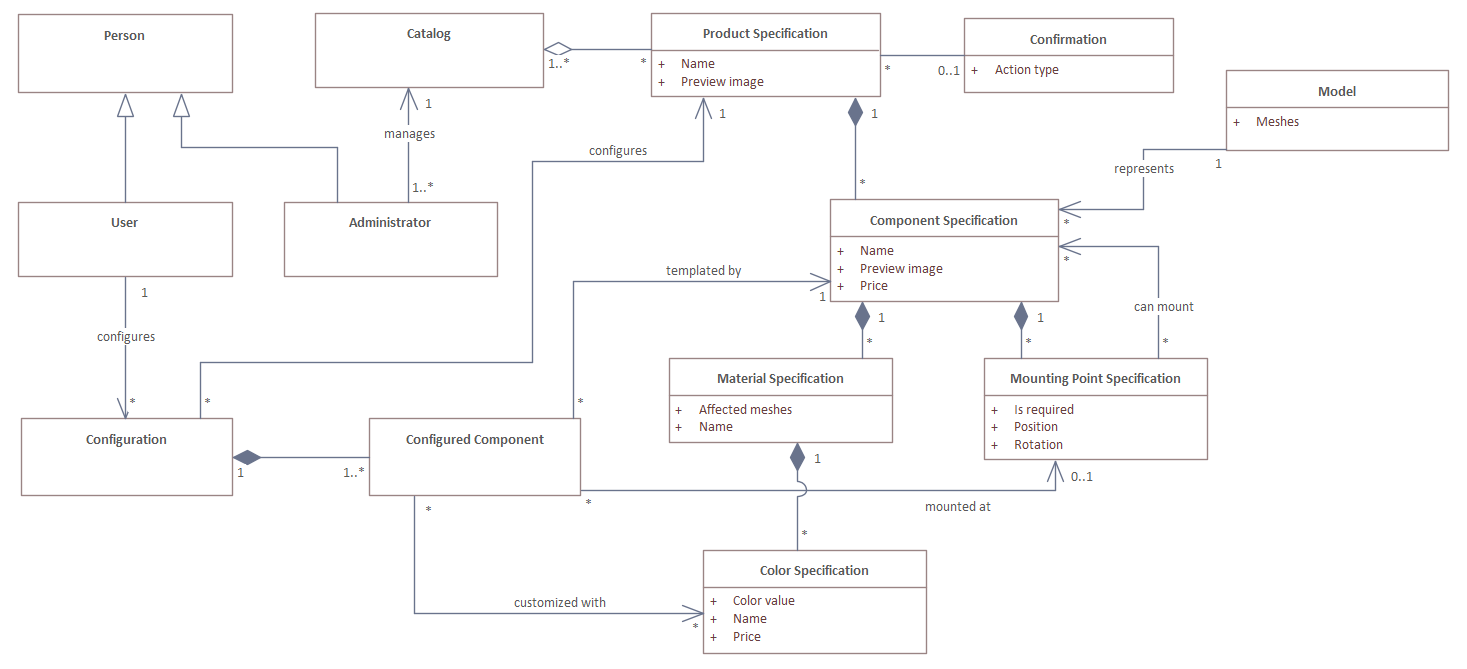
\includegraphics[width=\linewidth]{images/uml_domainmodel.png}
\caption{Domain model as a UML diagram}
\label{fig:domain-model}
\end{figure}
\end{landscape}

% - - - - - - - - - - - - - - - - - - - - - - - - - - - - - - -
\subsection{Catalog}
% - - - - - - - - - - - - - - - - - - - - - - - - - - - - - - -

The catalog forms the backbone of the proposed toolkit and defines the blueprint for customizable products. The catalog encompasses a variety of product specifications, each defining a configurable product along with all its potential customizations. This section delves into how these specifications lay the foundation for user-driven product configuration.
The entities discussed in this section are as follows:
\begin{itemize}[label=\rectanglebullet]
    \item Catalog
    \item Product Specification
    \item Component Specification
    \item Model
    \item Mounting Point Specification
    \item Material Specification
    \item Color Specification
    \item Administrator
\end{itemize}

A product specification acts as an overreaching comprehensive concept that encompasses all aspects of a given product. The entity may incorporate an action to finalize the configuration of the product, fulfilling the need for confirmation of the configuration (see requirement \hyperref[itm:F10]{F10}). Given that the tool focuses on the handling of modular products (see requirement \hyperref[itm:F3]{F3}), it is imperative that each product consists of various components. Therefore, the product specification is made up of component specifications, which represent all the various possible components that the product can have.

To meet the requirement of 3D visualization (see requirement \hyperref[itm:F3]{F3}), component specifications must be linked to a model featuring 3D meshes. This model acts as a representation of the component that will be presented to the user during the configuration process. In addition to this, the component specification is composed of material specifications and mounting point specifications.

Material specifications are needed with respect to the requirement of material color configuration (see requirement \hyperref[itm:F8]{F8}). They describe the materials of a given component that the user can customize, with each material specification providing mesh information specifying which part of the component this material influences, thereby enabling preview updates as the user makes selections. In addition, the material specification consists of color specifications that define the possible colors this material can take on in the configuration process.

Mounting point specifications are introduced to address the requirement of fixed point component placement (see requirement \hyperref[itm:F6]{F6}). They represent points on a component to which other modular components can be attached. The specifications of mounting point include the relative position and rotation of the point, the requirement for a component's presence at this point, and possible specifications of components that can be mounted on the point.

All these specifications are maintained in the catalog by the application administrator, who has the authority to modify any properties. The tool then utilizes these specifications to enable the configuration of tangible products.


% - - - - - - - - - - - - - - - - - - - - - - - - - - - - - - -
\subsection{Configuration}
% - - - - - - - - - - - - - - - - - - - - - - - - - - - - - - -

Transitioning from potential to actual, the configuration section delves into how users bring customizable products to life through the toolkit.
It illustrates how configured components are the building blocks of user-generated configurations, embodying the transformation from a generic template into a product uniquely tailored to individual preferences.
The entities covered in this section include:
\begin{itemize}[label=\rectanglebullet]
    \item Configuration
    \item Configured Component
    \item User
\end{itemize}

Users of the application create configurations. The cornerstone of a configuration lies in its configured components. The specifications described in the previous section serve as templates for these configured components. While the specifications outline all the configuration options, a configured component indicates a particular option selected by the user. Beyond the base component specification, a configured component also stores the mounting point to which it is attached, as well as the selected colors of its materials. Thus, a configuration is composed entirely of these individually configured components.


%______________________________________________________________
\section{User interface}
%---------------------------------------------------------------

The design of the user interface plays an essential part in the development of such a tool because it significantly influences user satisfaction when interacting with the tool. Good preparation of user interface design helps to determine the direction and streamline the implementation, as well as making clear from the beginning how to deal with factors such as responsiveness (see requirement \hyperref[itm:NF2]{NF2})

In this section, low-fidelity wireframes are used to depict the proposed user interface, highlighting the layout and architecture of the application. This approach captures the most important information at this stage, leaving the finer details to be refined as part of the implementation phase.

The design is based on the analysis of existing solutions and respects the design principles of similar solutions that are most intuitive and the users may already feel familiar with.

The configurator as an application is specific in that it primarily centers around the configuration process, with this interface being the most important and all other interfaces being secondary. In this section, the design of this configuration screen will be introduced, as well as the introductory and confirmation screens.

The common element of all screens is the top bar with the logo of the business that operates the configurator, which should redirect the user to the main website of the company when clicked. All of this should be customizable in the admin settings of the application.

% - - - - - - - - - - - - - - - - - - - - - - - - - - - - - - -
\subsection{Configuration screen}
% - - - - - - - - - - - - - - - - - - - - - - - - - - - - - - -

\begin{figure}[h]
\centering
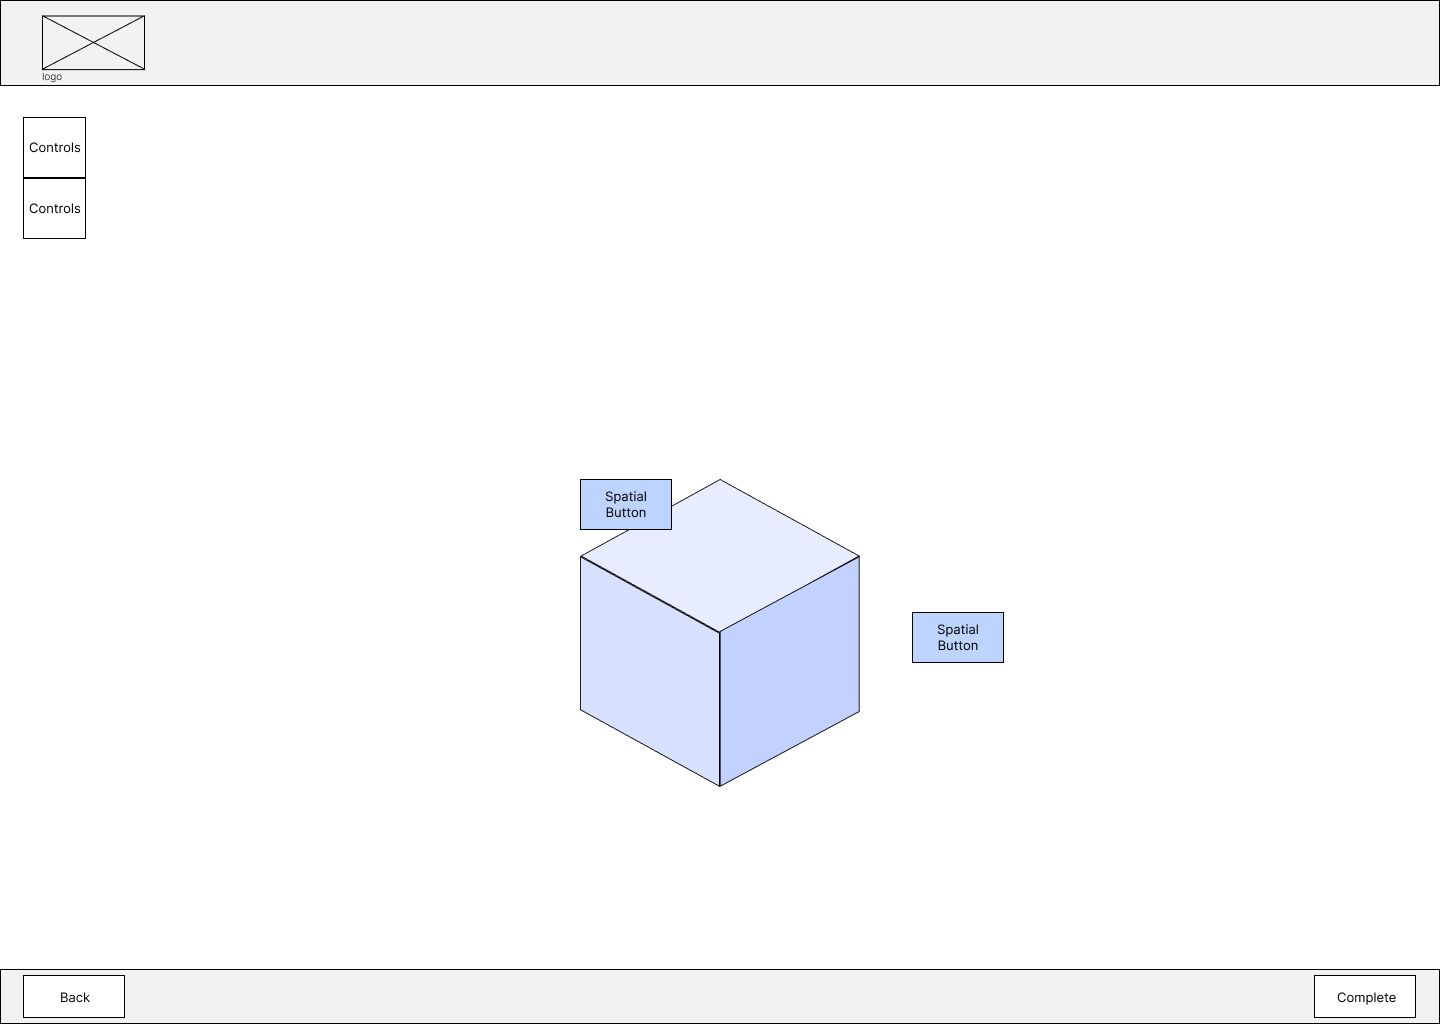
\includegraphics[width=0.7\textwidth]{images/wireframe_configuration_default.png}
\caption{Wireframe of configuration screen}
\label{fig:wireframe-configuration}
\end{figure}

The configuration screen is presented to the user during the configuration process. The screen is dominated by the 3D preview of the configured product, featuring interactable components and spatial buttons for the addition of components into the configuration. Control buttons are placed in the upper left corner within the 3D preview, symbolizing their direct relation to the preview, yet maintaining their distinctiveness as a separate element. At the bottom of the screen, there is another bar, this one containing buttons that allow users to go back or to finalize the configuration. The wireframe of the configuration screen in its default state is shown in  \autoref{fig:wireframe-configuration}, where the 3D preview of the product is represented by a blueish cube.

\begin{figure}[h]
\centering
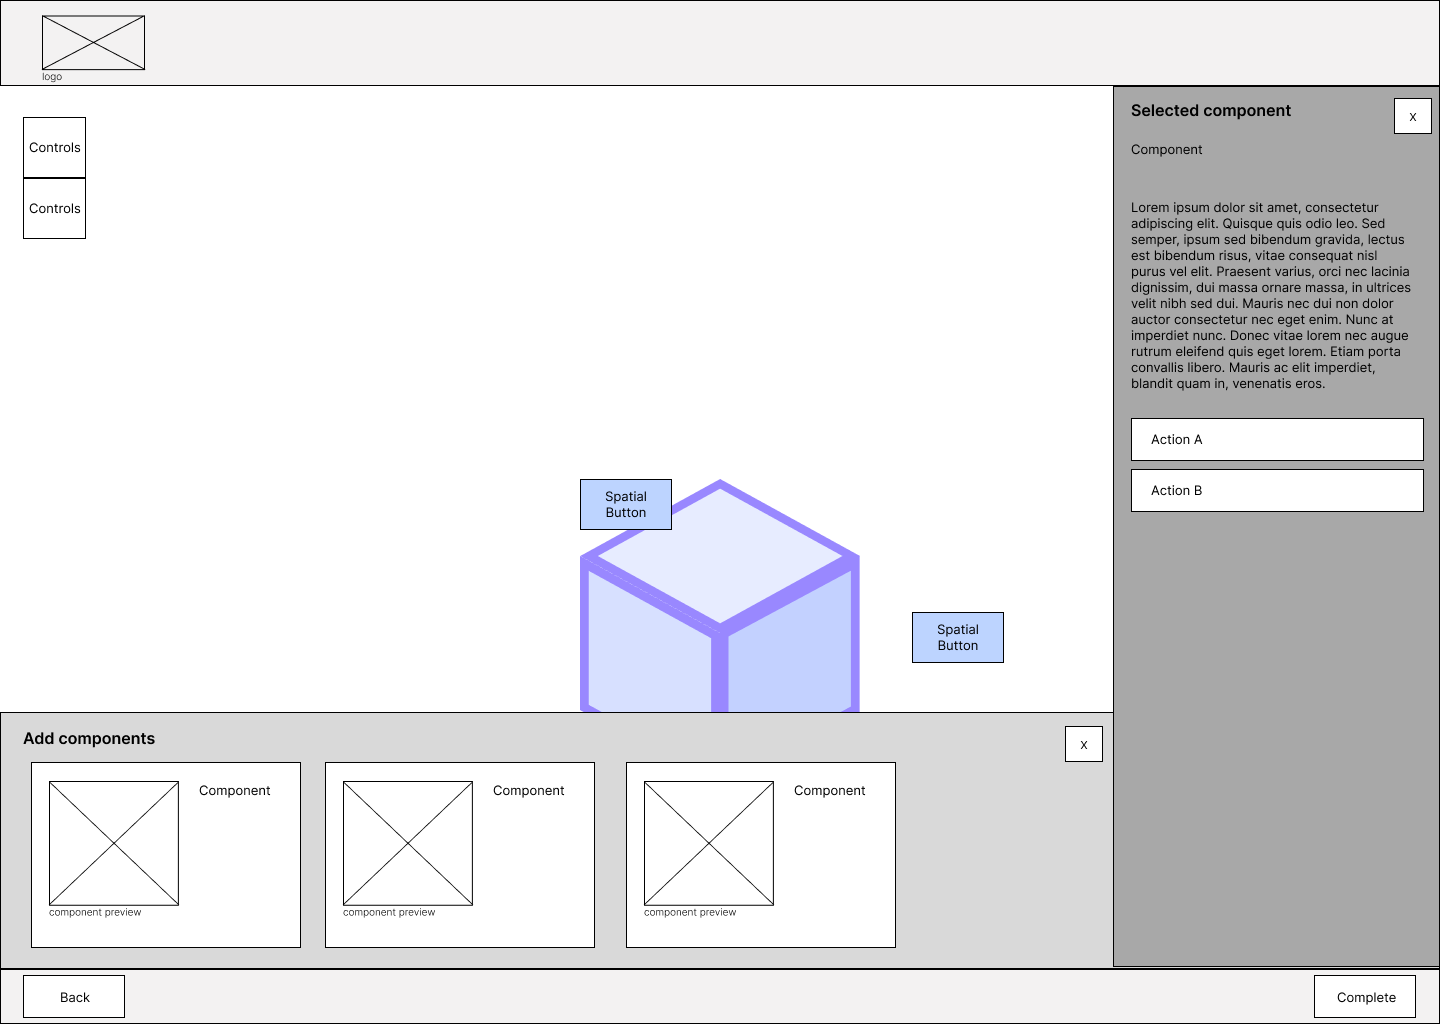
\includegraphics[width=0.7\textwidth]{images/wireframe_configuration_panels.png}
\caption{Wireframe of configuration screen with panels}
\label{fig:wireframe-configuration-panels}
\end{figure}

This default view, as outlined in the previous paragraph, maximizes the viewport with the most important presentation, which is the 3D preview of the product. However, at some stages of the configuration process, it is also necessary to present the user with further information. Therefore, upon selecting a component within the 3D preview, the component should become highlighted and, following the approach of existing solutions analyzed, a side panel with detailed information about the selected component will emerge from the right. If necessary, another panel with further options presented to the user may appear at the bottom. This design strategy maximizes the screen space for the important elements while still being flexible enough to present additional information in a streamlined way. The wireframe of the interface with panels that contain additional information and options presented is shown in \autoref{fig:wireframe-configuration-panels}.

\begin{figure}[h]
    \centering
    \begin{minipage}{0.4\textwidth}
        \centering
        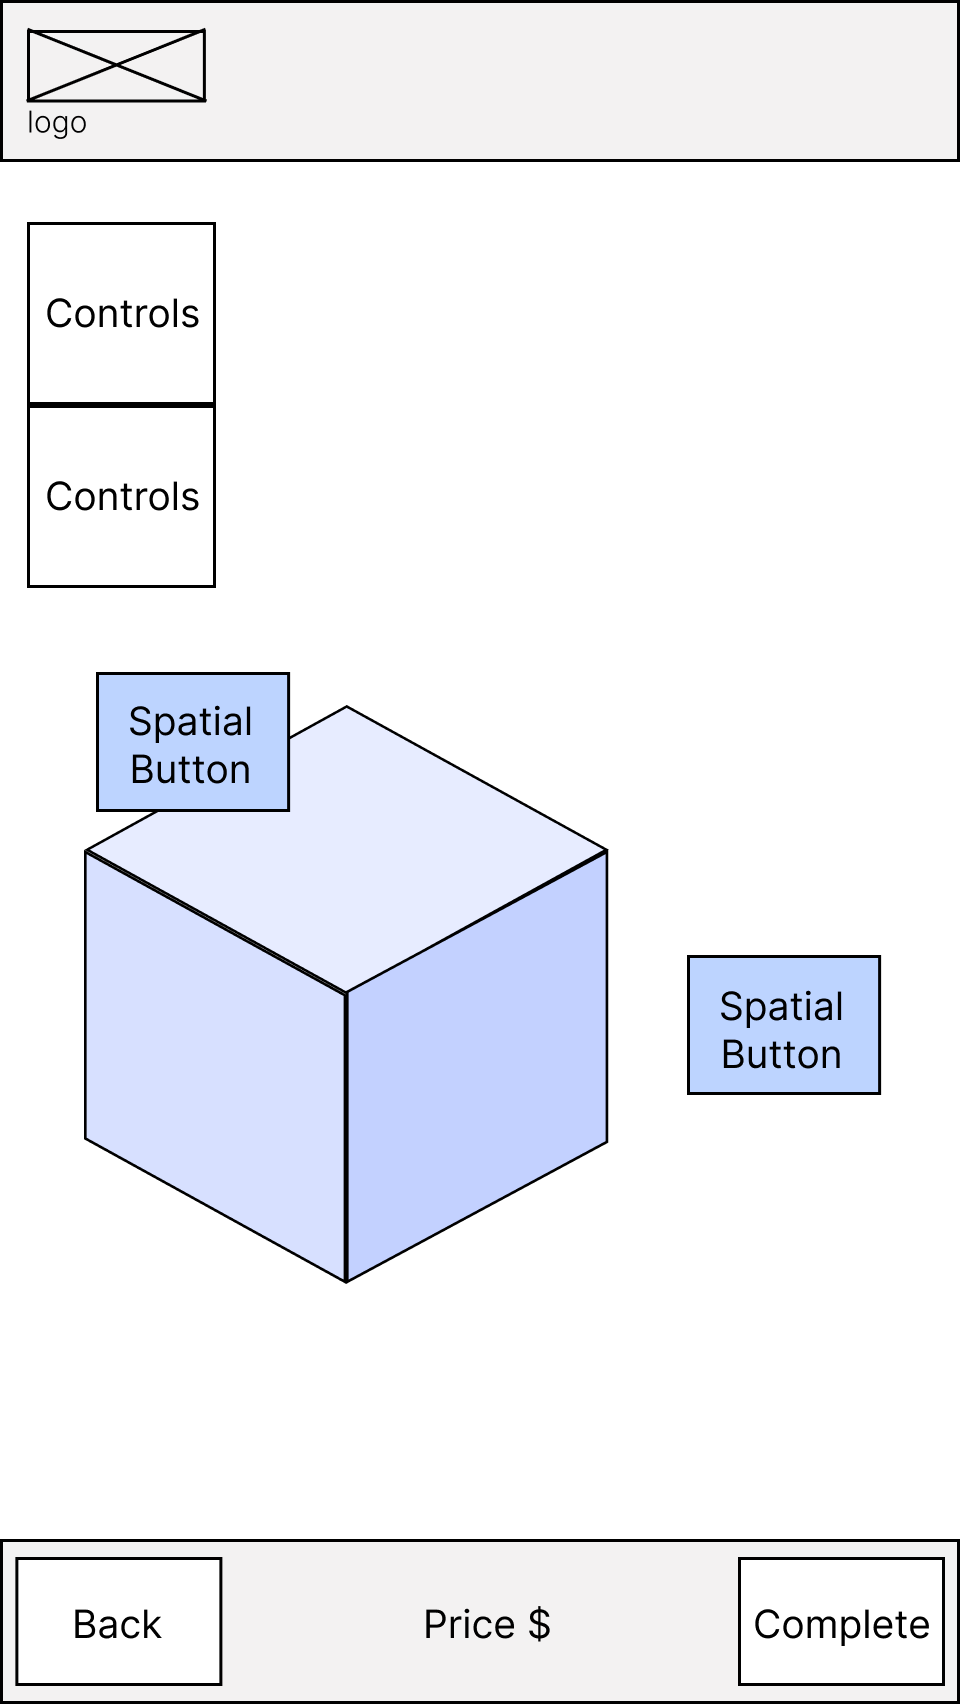
\includegraphics[width=\linewidth]{images/wireframe_configuration_mobile_default.png}
        \caption{Wireframe of mobile configuration screen}
        \label{fig:wireframe-configuration-mobile}
    \end{minipage}\hfill
    \begin{minipage}{0.4\textwidth}
        \centering
        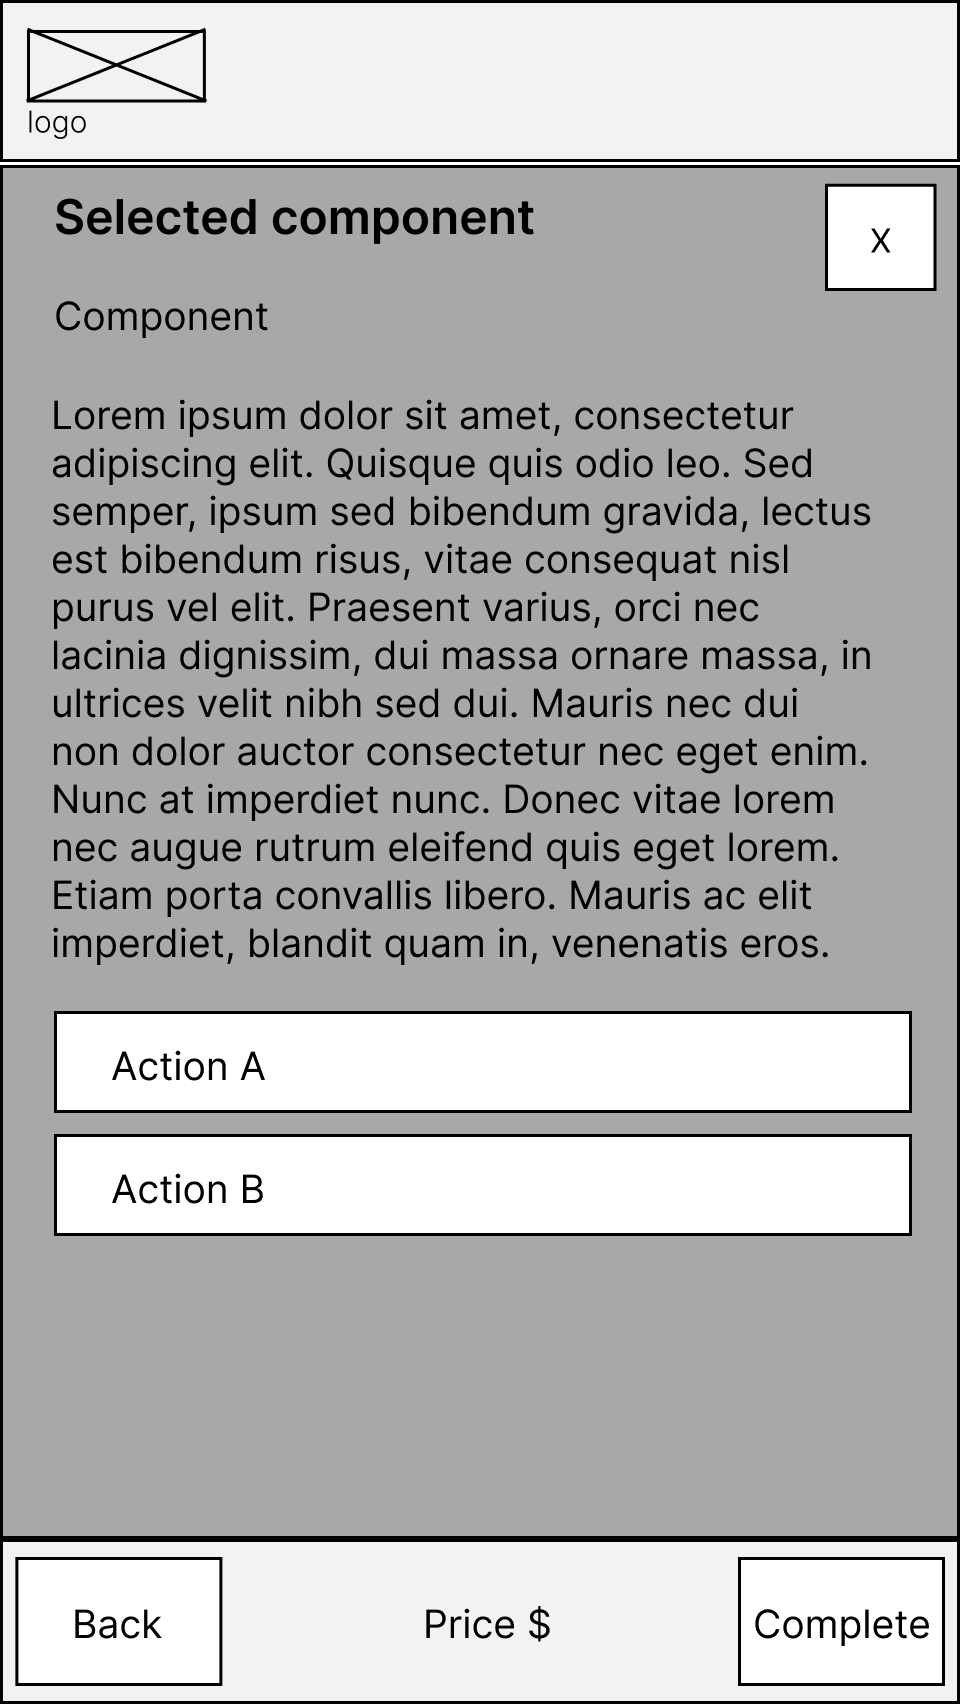
\includegraphics[width=\linewidth]{images/wireframe_configuration_mobile_panels.png}
        \caption{Wireframe of mobile configuration screen with panels}
        \label{fig:wireframe-configuration-panel-mobile}
    \end{minipage}
\end{figure}

To ensure responsiveness, a mobile version of the interface should also be outlined. The prioritization of the 3D preview in the default state makes this simple, as this just means that on smaller viewports the elements are presented in the same way, with the preview being in different aspect ratio, which is easily compensated by the 3D preview taking on different zoom level. The outline of this wireframe is presented in \autoref{fig:wireframe-configuration-mobile}.

The wireframe for the mobile version of the interface with the presented detail side panel is shown in \autoref{fig:wireframe-configuration-panel-mobile}. At this reduced viewport size, the side panel can maintain the same internal layout but to be usable it needs to occupy the whole 3D preview. This will need to be kept in mind when utilizing interactions with the 3D preview, as it may not always be fully visible when the panels are active. 

The design remains mostly consistent on both small and large viewports, while still being adaptive and responsive. This ensures that the familiarity with the tool is maintained for all viewport sizes.

% - - - - - - - - - - - - - - - - - - - - - - - - - - - - - - -
\subsection{Introduction screen}
% - - - - - - - - - - - - - - - - - - - - - - - - - - - - - - -

\begin{figure}[h]
\centering
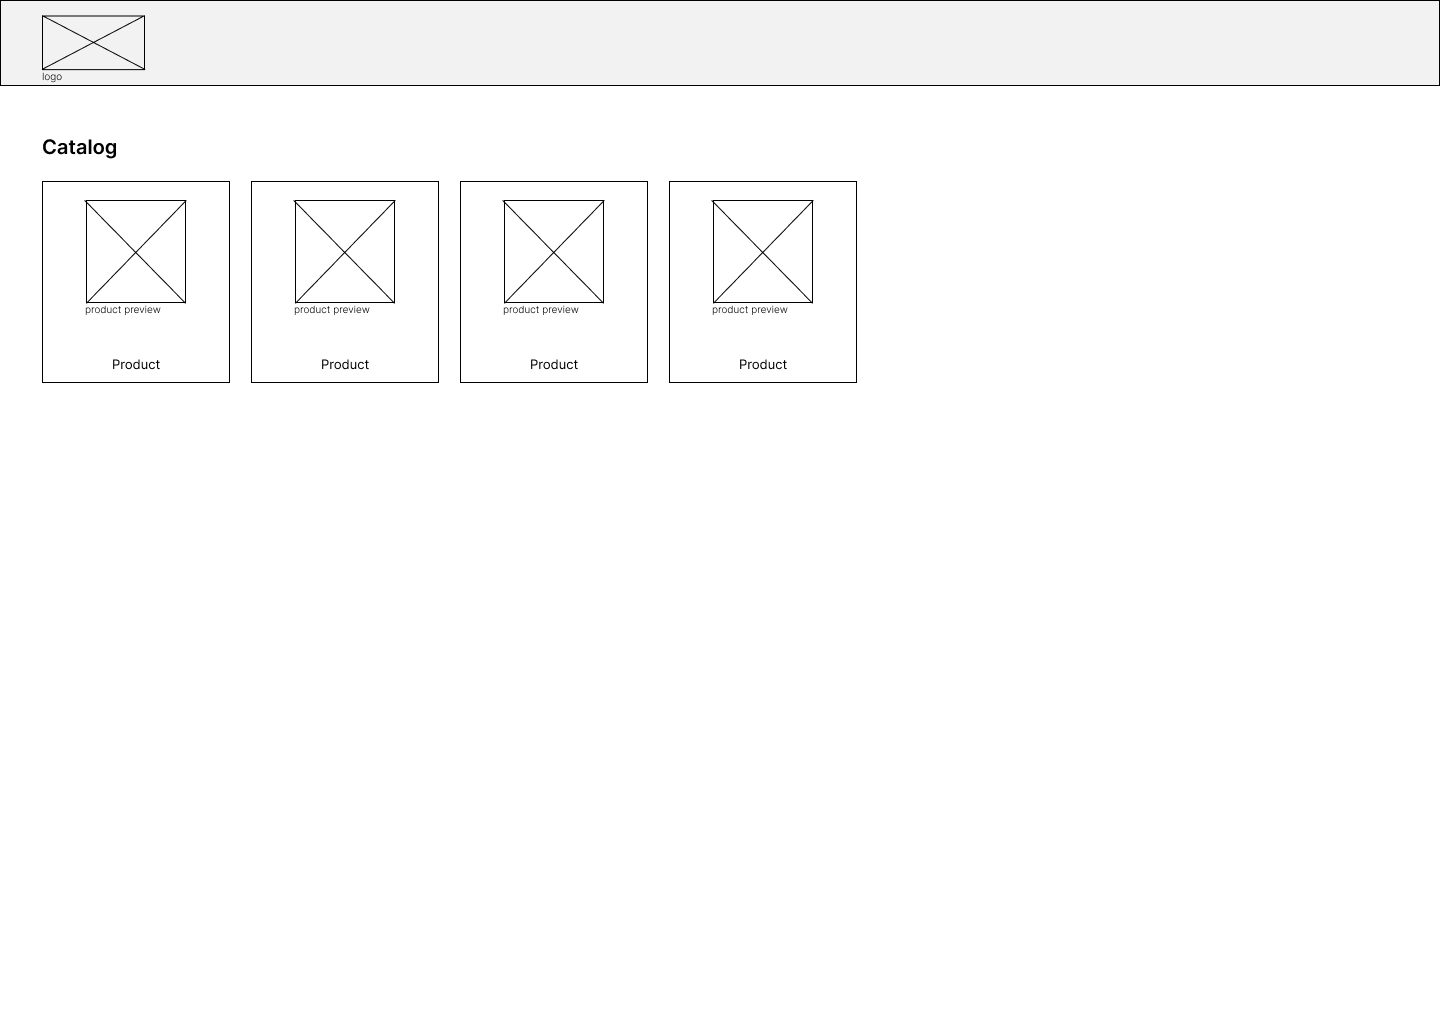
\includegraphics[width=0.7\textwidth]{images/wireframe_introduction_default.png}
\caption{Wireframe of introduction screen}
\label{fig:wireframe-introduction}
\end{figure}

The introduction screen is the first screen presented to the user when launching the application. It offers a simple way of selecting the configurable product from the catalog, with image and name of the product presented on a large tile. The selection of the product takes the user to the configuration process. Mobile interface of this screen mirrors the large version. The wireframe of the design can be seen in \autoref{fig:wireframe-introduction}.

% - - - - - - - - - - - - - - - - - - - - - - - - - - - - - - -
\subsection{Confirmation screen}
% - - - - - - - - - - - - - - - - - - - - - - - - - - - - - - -

\begin{figure}[hb]
\centering
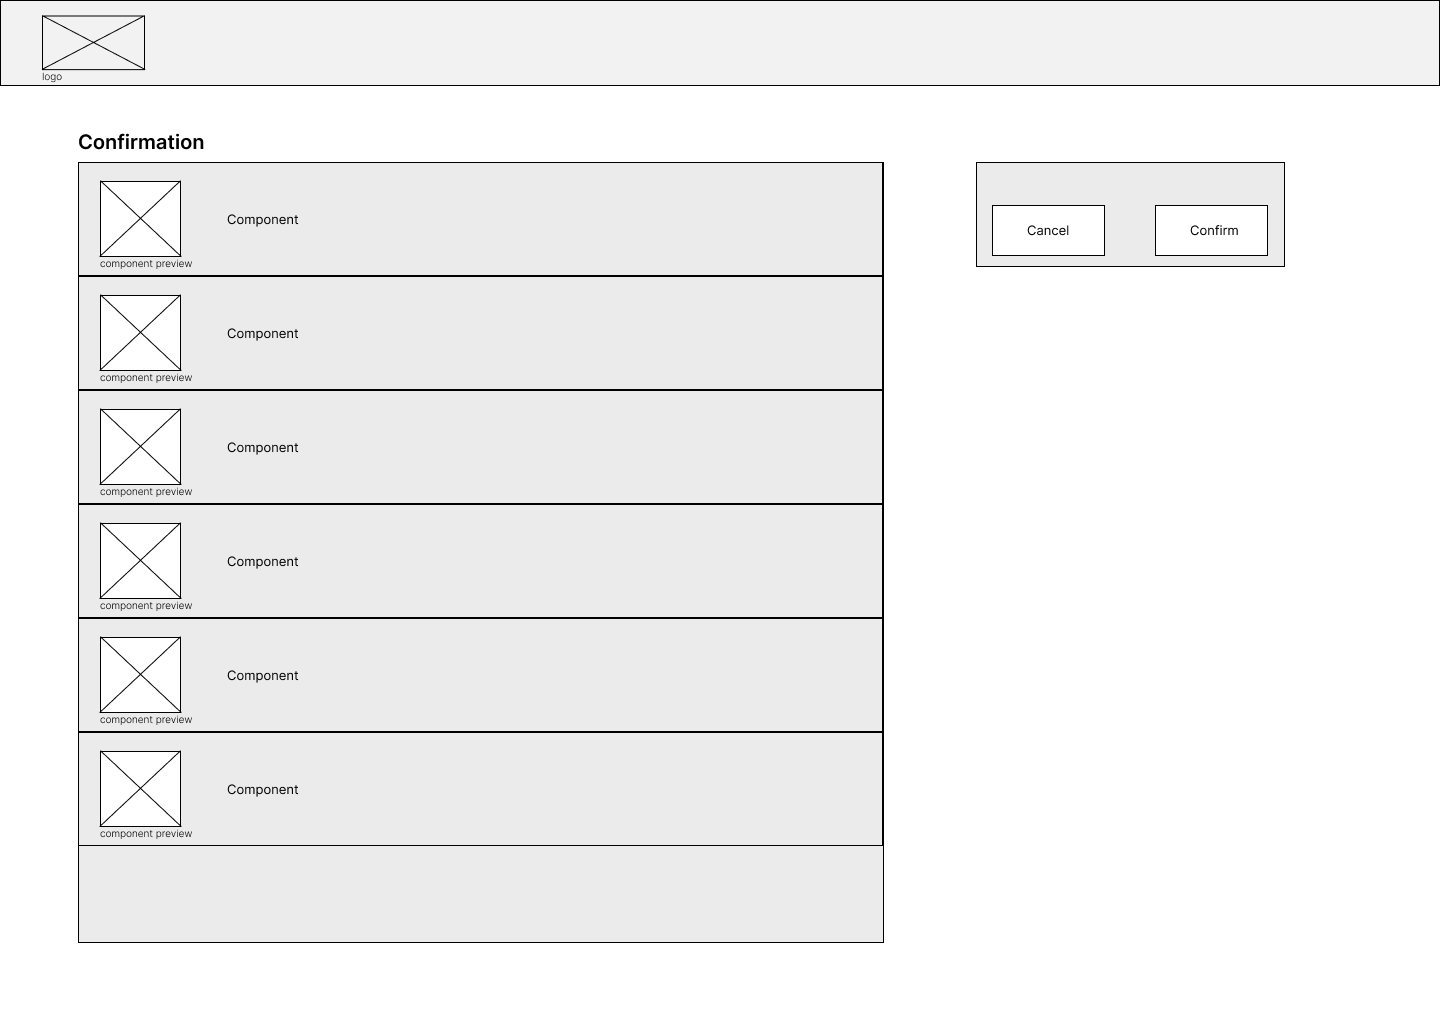
\includegraphics[width=0.7\textwidth]{images/wireframe_confirmation_default.png}
\caption{Wireframe of confirmation screen}
\label{fig:wireframe-confirmation}
\end{figure}

The confirmation screen is presented to the user at the end of the configuration and satisfies the configuration review requirement (see requirement \hyperref[itm:F9]{F9}). The wireframe of the configuration screen is shown in \autoref{fig:wireframe-confirmation}. On the left side, the confirmation screen presents the selected and configured components in a comprehensive list and allows the user to review their choices. The right side of the screen contains two buttons, one to confirm the configuration, which can initiate the confirmation action, and another to return to the configuration process for any adjustments. 

\begin{figure}[h]
\centering
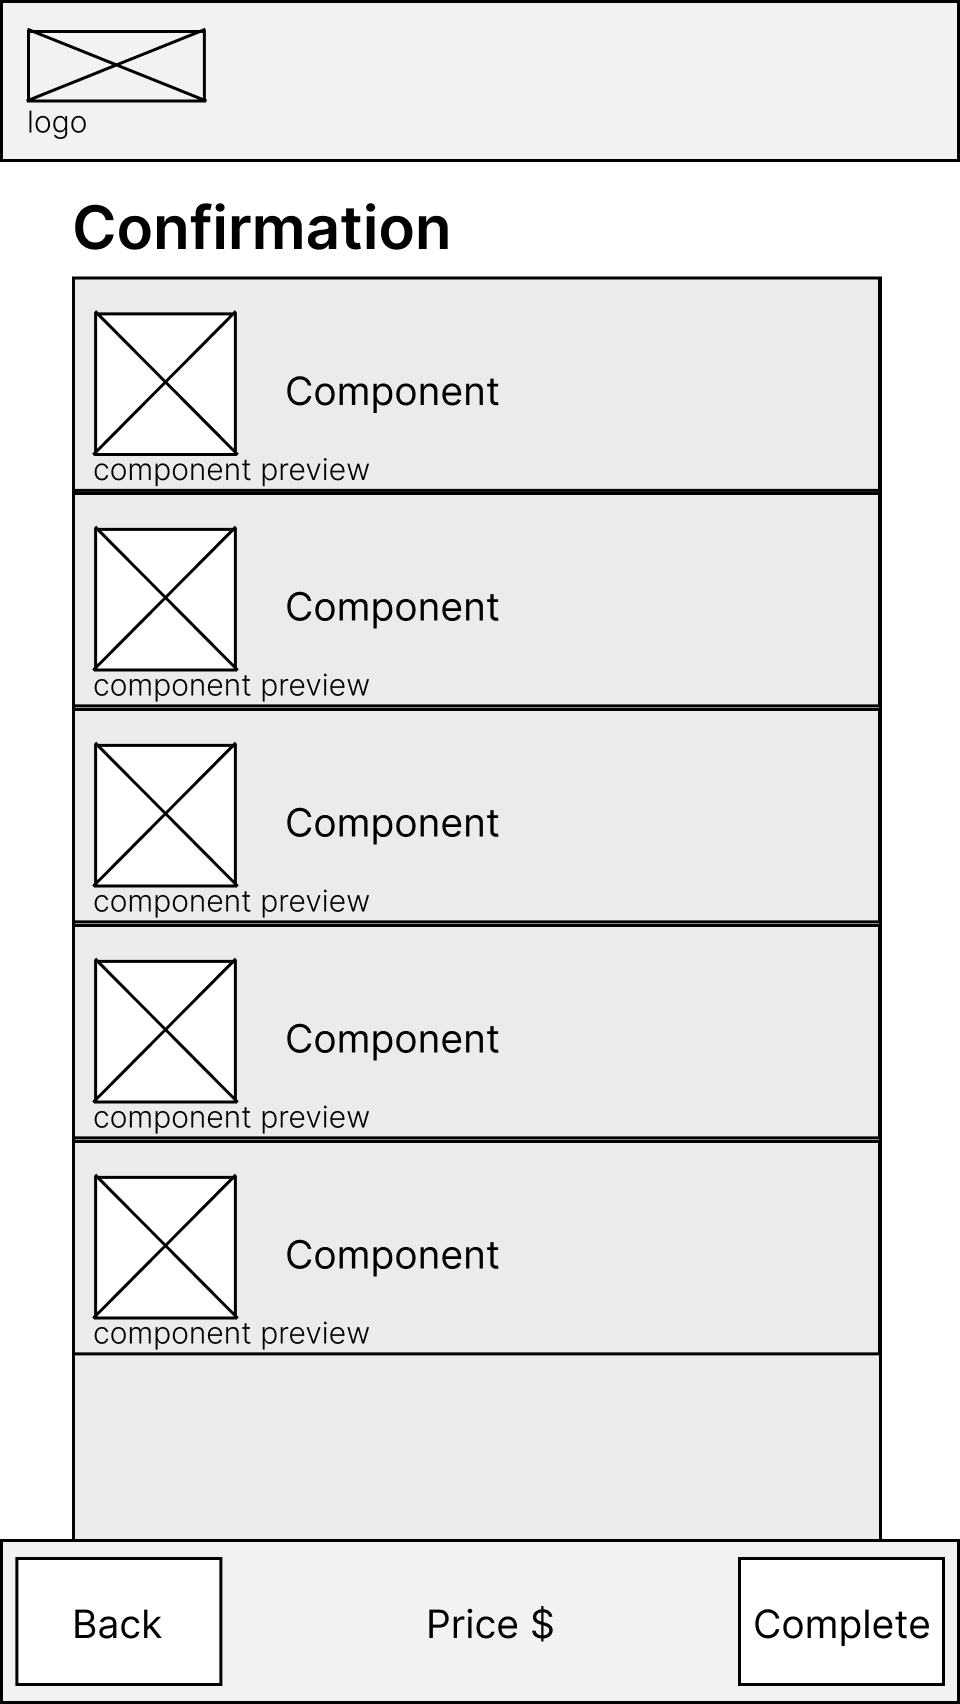
\includegraphics[width=0.3\textwidth]{images/wireframe_confirmation_mobile_default.png}
\caption{Wireframe of mobile confirmation screen}
\label{fig:wireframe-confirmation-mobile}
\end{figure}

The wireframe for the mobile version of the confirmation screen is depicted in  \autoref{fig:wireframe-confirmation-mobile}. In this layout, the summary spans the entire width of the screen, with the buttons moved to form a bar at the bottom of the screen.

\todo{Add prices to the wireframes and images and names to the domain model.}

% Do not forget to include Introduction
%---------------------------------------------------------------
% \chapter{Introduction}
% uncomment the following line to create an unnumbered chapter
\chapter*{Introduction}\addcontentsline{toc}{chapter}{Introduction}\markboth{Introduction}{Introduction}
%---------------------------------------------------------------
\setcounter{page}{1}

% The following environment can be used as a mini-introduction for a chapter. Use that anyway it pleases you (or comment it out). It can contain, for instance, a summary of the chapter. Or, there can be a quotation.
\begin{chapterabstract}
	Product configurators and their value.
\end{chapterabstract}

Over the past few decades, the rise of e-commerce has caused a shift in consumer expectations, resulting in an increased demand for customized products. This gives rise to the need to shift focus towards mass customization, where products are customized according to individual preferences. To thrive in this sector, companies must modify their product offerings to be able to meet the unique needs of users. This necessitates the existence of a system (a toolkit), that enables customers to express their preferences and convert them into product configurations. \cite{Fulkerson2000}

The introduction of customization has been shown to significantly improve the customer's perception of the product's value. The involvement of consumers in the customization process leads to a stronger bond with the product, resulting in a perception of higher value compared to standard off-the-shelf products. This aspect of mass customization makes it an appealing and compelling strategy for businesses to implement. \cite{Schreier2006} However, when implementing such a system, it is crucial to ensure that the customization process is pleasurable for the customer. Research has shown that the enjoyment experienced during the customization also affects the perceived value of the final product, highlighting the importance of good implementation. \cite{Franke2010}

The task of transforming user preferences into concrete designs is a difficult endeavor that can be further hindered by a lack of effective communication between the customer's explanation of their desires and the business's comprehension. The use of online product configurators seemingly provides a solution for this issue by offering a user-friendly and visually appealing platform, which allows customers to customize products to their specifications, improves customer experience by increasing engagement and interactivity, and helps to bridge the gap between customer expectations and the end product. These tools have become an integral part of successful personalization strategies. \cite{Franke2003}

The introduction of modern technologies such as WebGL or Augmented Reality (AR) has expanded the potential of online configurators. These advances enable these toolkits to become more powerful and visually illustrative tools that provide a higher level of interactivity and realism than what was previously accessible. \cite{Cozzi2015}

%---------------------------------------------------------------
\section{Objective of this thesis}
%---------------------------------------------------------------

The primary objective of this thesis is to design and implement an application (toolkit) for the online configuration of modular products. The toolkit aims to be product-agnostic, adaptable, and customizable, usable by a variety of businesses, enabling their customers to interactively customize their modular products. The focus is on ensuring that the toolkit is not only flexible in accommodating various specific needs, but also straightforward for businesses to maintain after deploying, emphasizing lightweight infrastructure requirements. 
To accomplish this main objective, this requires an analysis of the characteristics found in current product configurators, as well as an examination of comparable solutions currently available to businesses.

%---------------------------------------------------------------
\section{Structure of this thesis}
%---------------------------------------------------------------

This thesis is divided into six chapters.

\begin{description}
\item[Chapter 1] The initial chapter entails an examination of existing solutions and an investigation into the functionalities that should be incorporated into this particular application.

\item[Chapter 2] The second chapter discusses the design of the application, the technologies chosen, the architecture, and the data structures.

\item[Chapter 3] The third chapter is devoted to implementation.

\item[Chapter 4] Chapter four focuses on the deployment of the implemented application in a particular business as an example. In addition, it discusses the resulting changes in the business processes of the selected business.

\item[Chapter 5] In the fifth chapter, the tests used in the development of the application are described.

\item[Chapter 6] Finally, the last chapter summarizes the results achieved and suggests possible directions for future development.
\end{description}


%---------------------------------------------------------------
\chapter{Analysis}
%---------------------------------------------------------------

\begin{chapterabstract}
	Lorem ipsum dolor sit amet. 
\end{chapterabstract}

Product configurators can be implemented in various ways, and the design of the tool itself determines the types of products that can be designed using the tool later on. The number of different unique configurations of a product that the tool can create is called the solution space. The size of the solution space is determined by two factors: the number of customizable attributes and the achievable values of each attribute. \cite{Huiwen2018} A relevant study examines the solution spaces of these toolkits and proposes an evaluation model that enables the categorization and assessment of various implementation approaches. Based on the target outcome and the guidance provided by the tool, the following mechanisms are specified: \cite{Hermans2012}

\begin{definition}[Veneer]
Customization by adding a visual decorative layer. (e.g. printing, engraving, etching)
\end{definition}
\begin{definition}[Modularity]
Customization by combining modules or components.
\end{definition}
\begin{definition}[Parametric]
Customization by changing the parameter values of parts.
\end{definition}
\begin{definition}[Generative]
Customization using code and scripting to synthesize the final form of the product.
\end{definition}

The main focus of this thesis is toolkits that primarily employ modularity mechanisms, however, there are often some common characteristics among configuration tools with different mechanisms.

\section{Exploring existing solutions}
\subsection{Configurators in use}

Currently, many companies are integrating product configurators into their sales strategies across multiple industries such as automotive, fashion, furniture, housing, and others. These configurators serve as either the main or supplementary sales tools for these businesses.

The Configurator Database Project by cyLEDGE MEDIA aims to catalog these web-based configuration tools. In the 2017/2018 report, they tracked 1250 deployments of these tools; however, the true count will be significantly higher since the database only includes the most frequently visited applications. \cite{cyLEDGE2018}

An analysis of the 100 most viewed configurators from May 2020 to May 2021 in the Configurator Database Project was performed in a study that examined the shared characteristics of these configurations. The results of some of the relevant characteristics and design choices that the study has analyzed are presented in this section: \cite{Blazek2023}
\begin{itemize}
    \item \textbf{Responsive design}: 75.3\% of examined tools had responsive design (the design adapted to the viewport of the device) 
    \item \textbf{Navigation}: 17.5\% of configurators had linear predefined navigation (meaning the configuration had to follow a specified sequence), whereas the majority of tools (82.5\%) had open navigation (user has the flexibility to configure the product in any order)
    \item \textbf{Visualization} 79.4\% of tools utilized photorealistic visualization (as opposed to illustrations or no visualization), however, the study acknowledges that there were significant variations based on the industries in which the configurator is utilized
    \item \textbf{Data transfer} The mean network data size transferred for 3D configurator was 35.6~MB
    \item \textbf{Configuration options} 60.8\% of configurators offered more than ten customizable attributes
    \item \textbf{Purchase capability} Given that car brands typically do not directly sell their cars online, it is logical to exclude them from the analysis of this particular characteristic. With the exclusion of vehicle configurators, 70.5\% of the configurators could complete an online purchase of the configured product
    \item \textbf{Price calculation} 56.7\% of the configurators were able to instantly reflect the changes made to the configuration in the displayed price
\end{itemize}

Another article also used the same database of configurators to analyze common design elements. They identified several key designs that were prevalent in the majority of configurators analyzed. The following key insights of common, recommended designs from the article are relevant to this thesis: \cite{Leitner2014}
\begin{itemize}
    \item At the end of the configuration process, a summary of selected options is presented
    \item To present the products that can be configured, images that are large enough to see details are used
    \item If the configurator has linear predefined navigation, the navigation information is presented on a horizontal plane
    \item Navigation bar is visible
    \item Price and order button is clearly visible and available for completion purposes
    \item Prices of the components are accessible in all phases of the configuration
    \item Logo is displayed prominently
    \item User preferences should be adaptable
\end{itemize}

As part of the analysis chapter of this thesis, it is essential to examine actual 3D~configurator applications. Due to the large number of existing applications, it is not within the scope of this work to perform an exhaustive analysis. Instead, this section will focus on a select group of four applications. These have been selected based on a combination of factors such as their popularity, functionality, and importance in the context of a modular product configuration. This selection is intended to provide insightful examples that highlight different approaches, rather than being representative of the entire domain.

\subsubsection{IKEA PAX planner tool}
\subsubsection{Lundia Original kastconfigurator}
\subsubsection{Muuto planner}
\subsubsection{LD Seating Nido}

\subsection{Offered toolkits}

\subsubsection{ThreeKit}
\subsubsection{Emersyea}
\subsubsection{Roomle} % include `text.tex' from `text/' subdirectory

\appendix\appendixinit % do not remove these two commands

\chapter{Additional visuals}

\begin{figure}
\centering
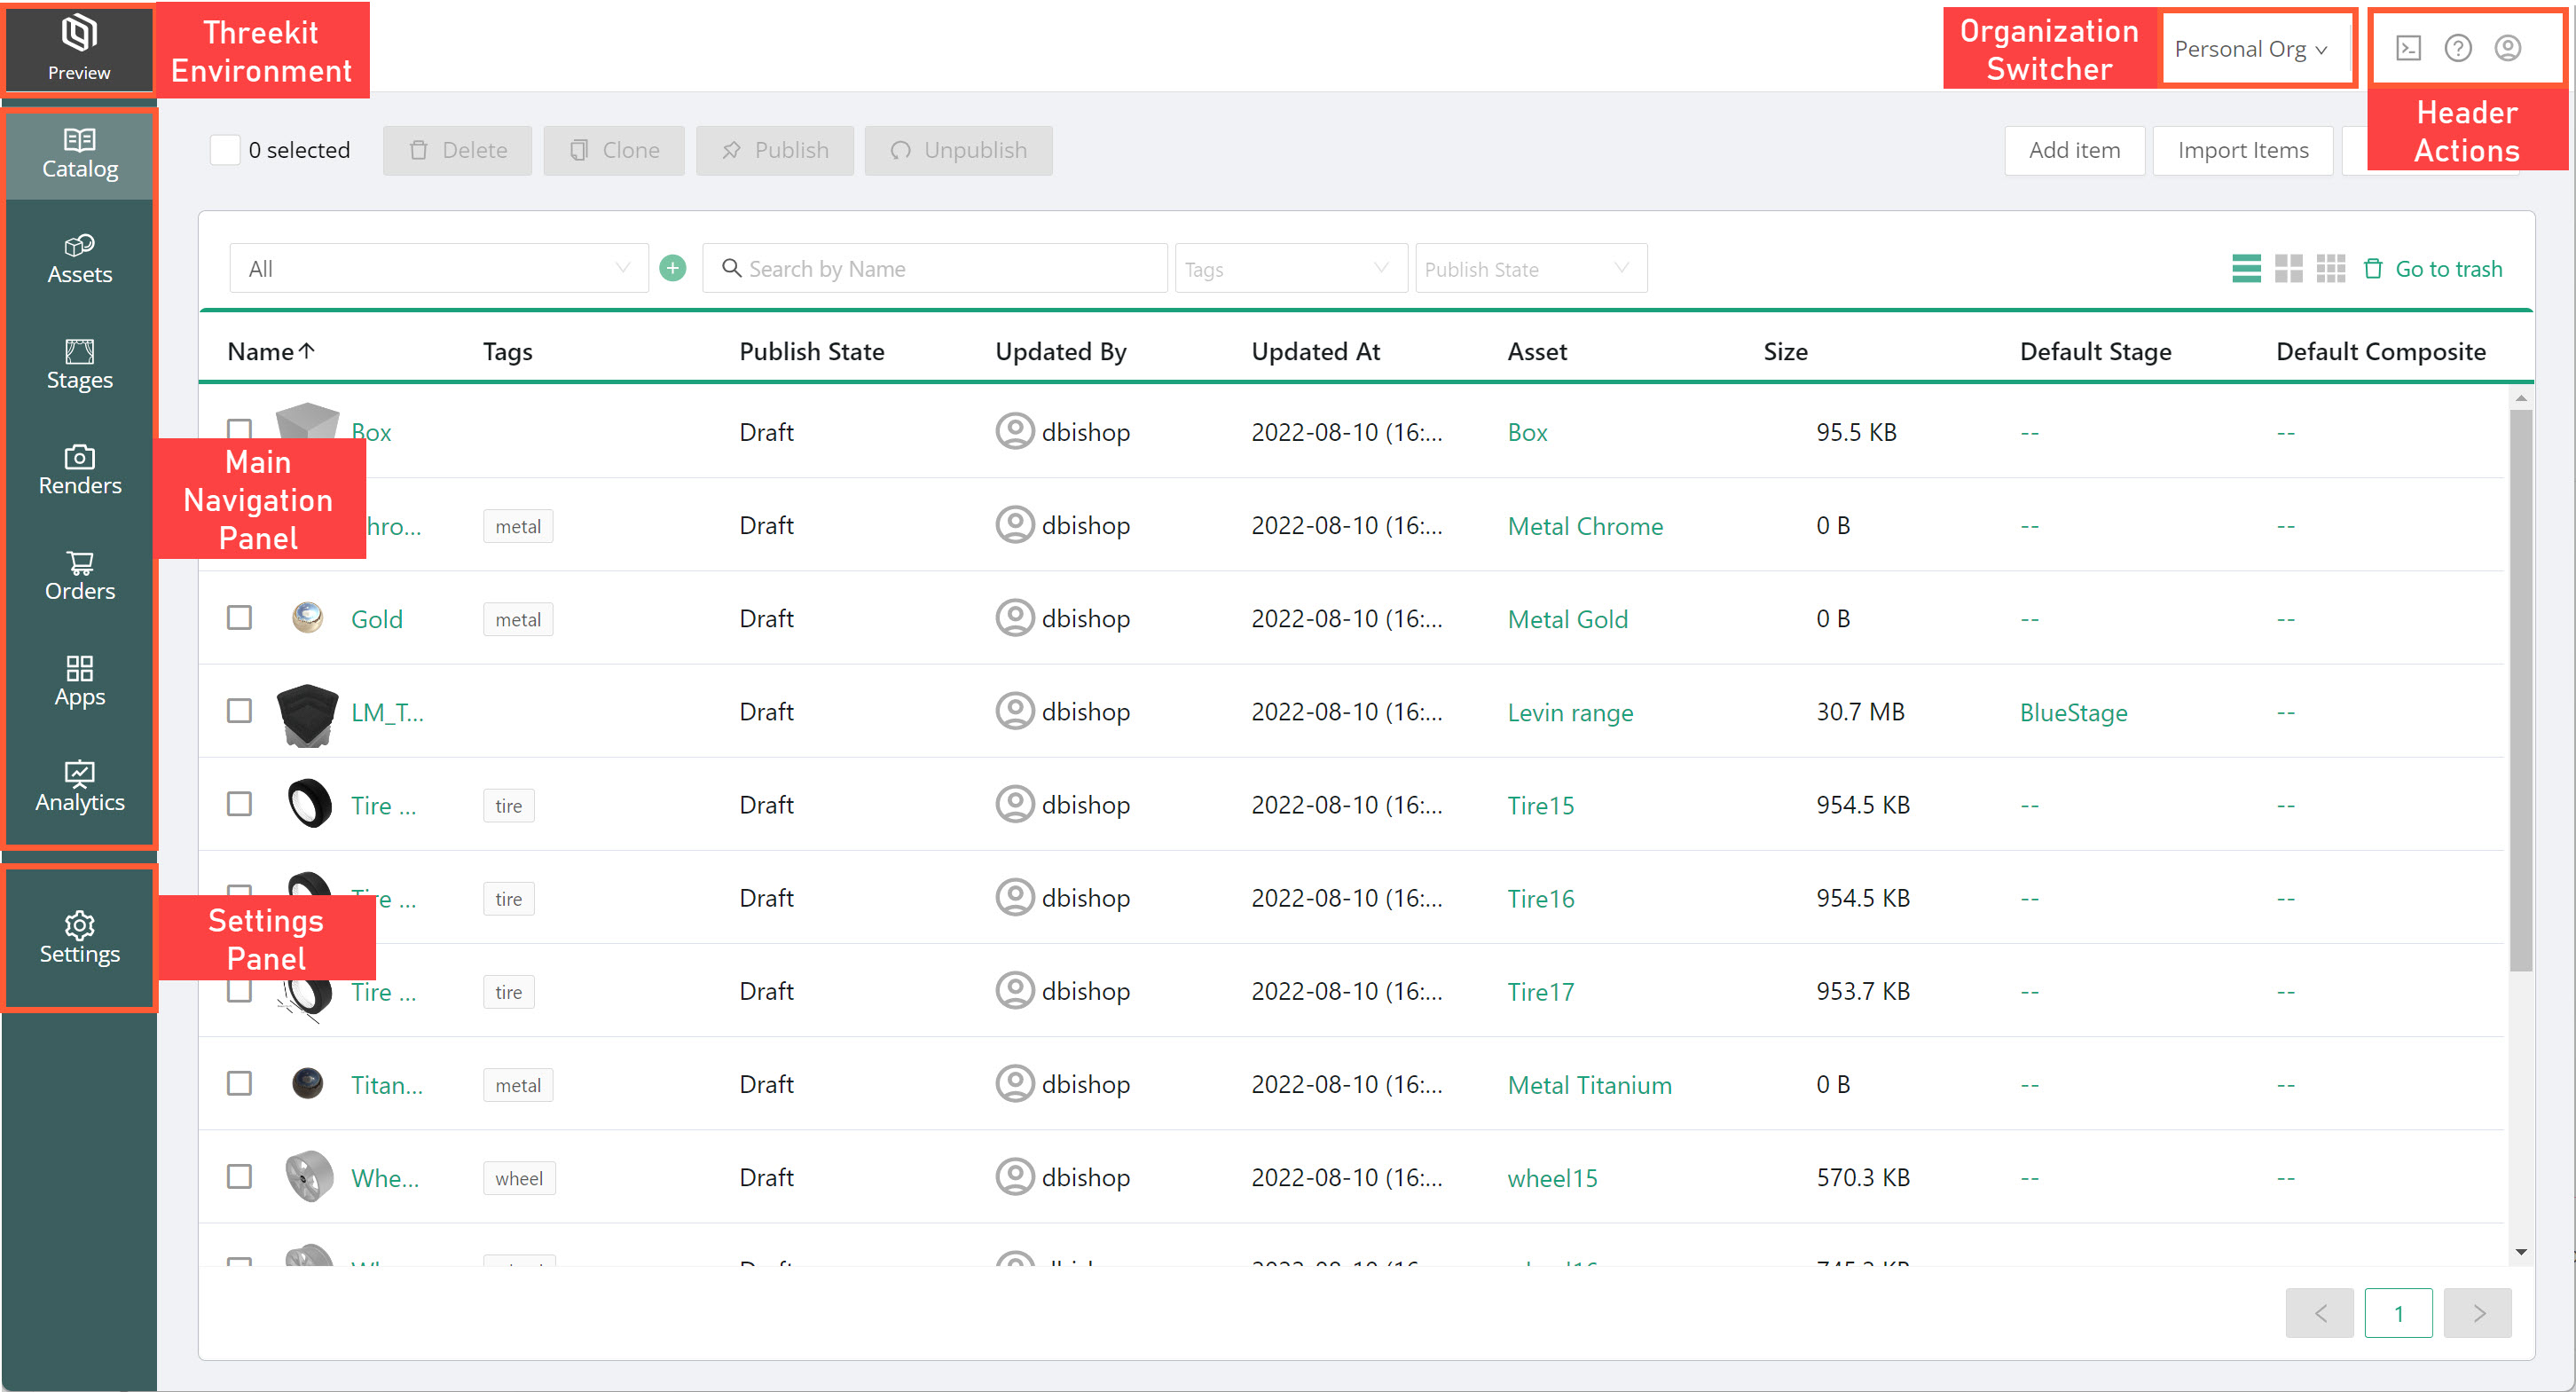
\includegraphics[width=14cm]{images/analysis_threekit-platform.jpg}
\captionsource{Threekit's Platform's landing page}{Threekit Platform Documentation \cite{ThreeKitPlatformDocumentation}}
\label{fig:threekit-platform}
\end{figure}

\begin{figure}
\centering
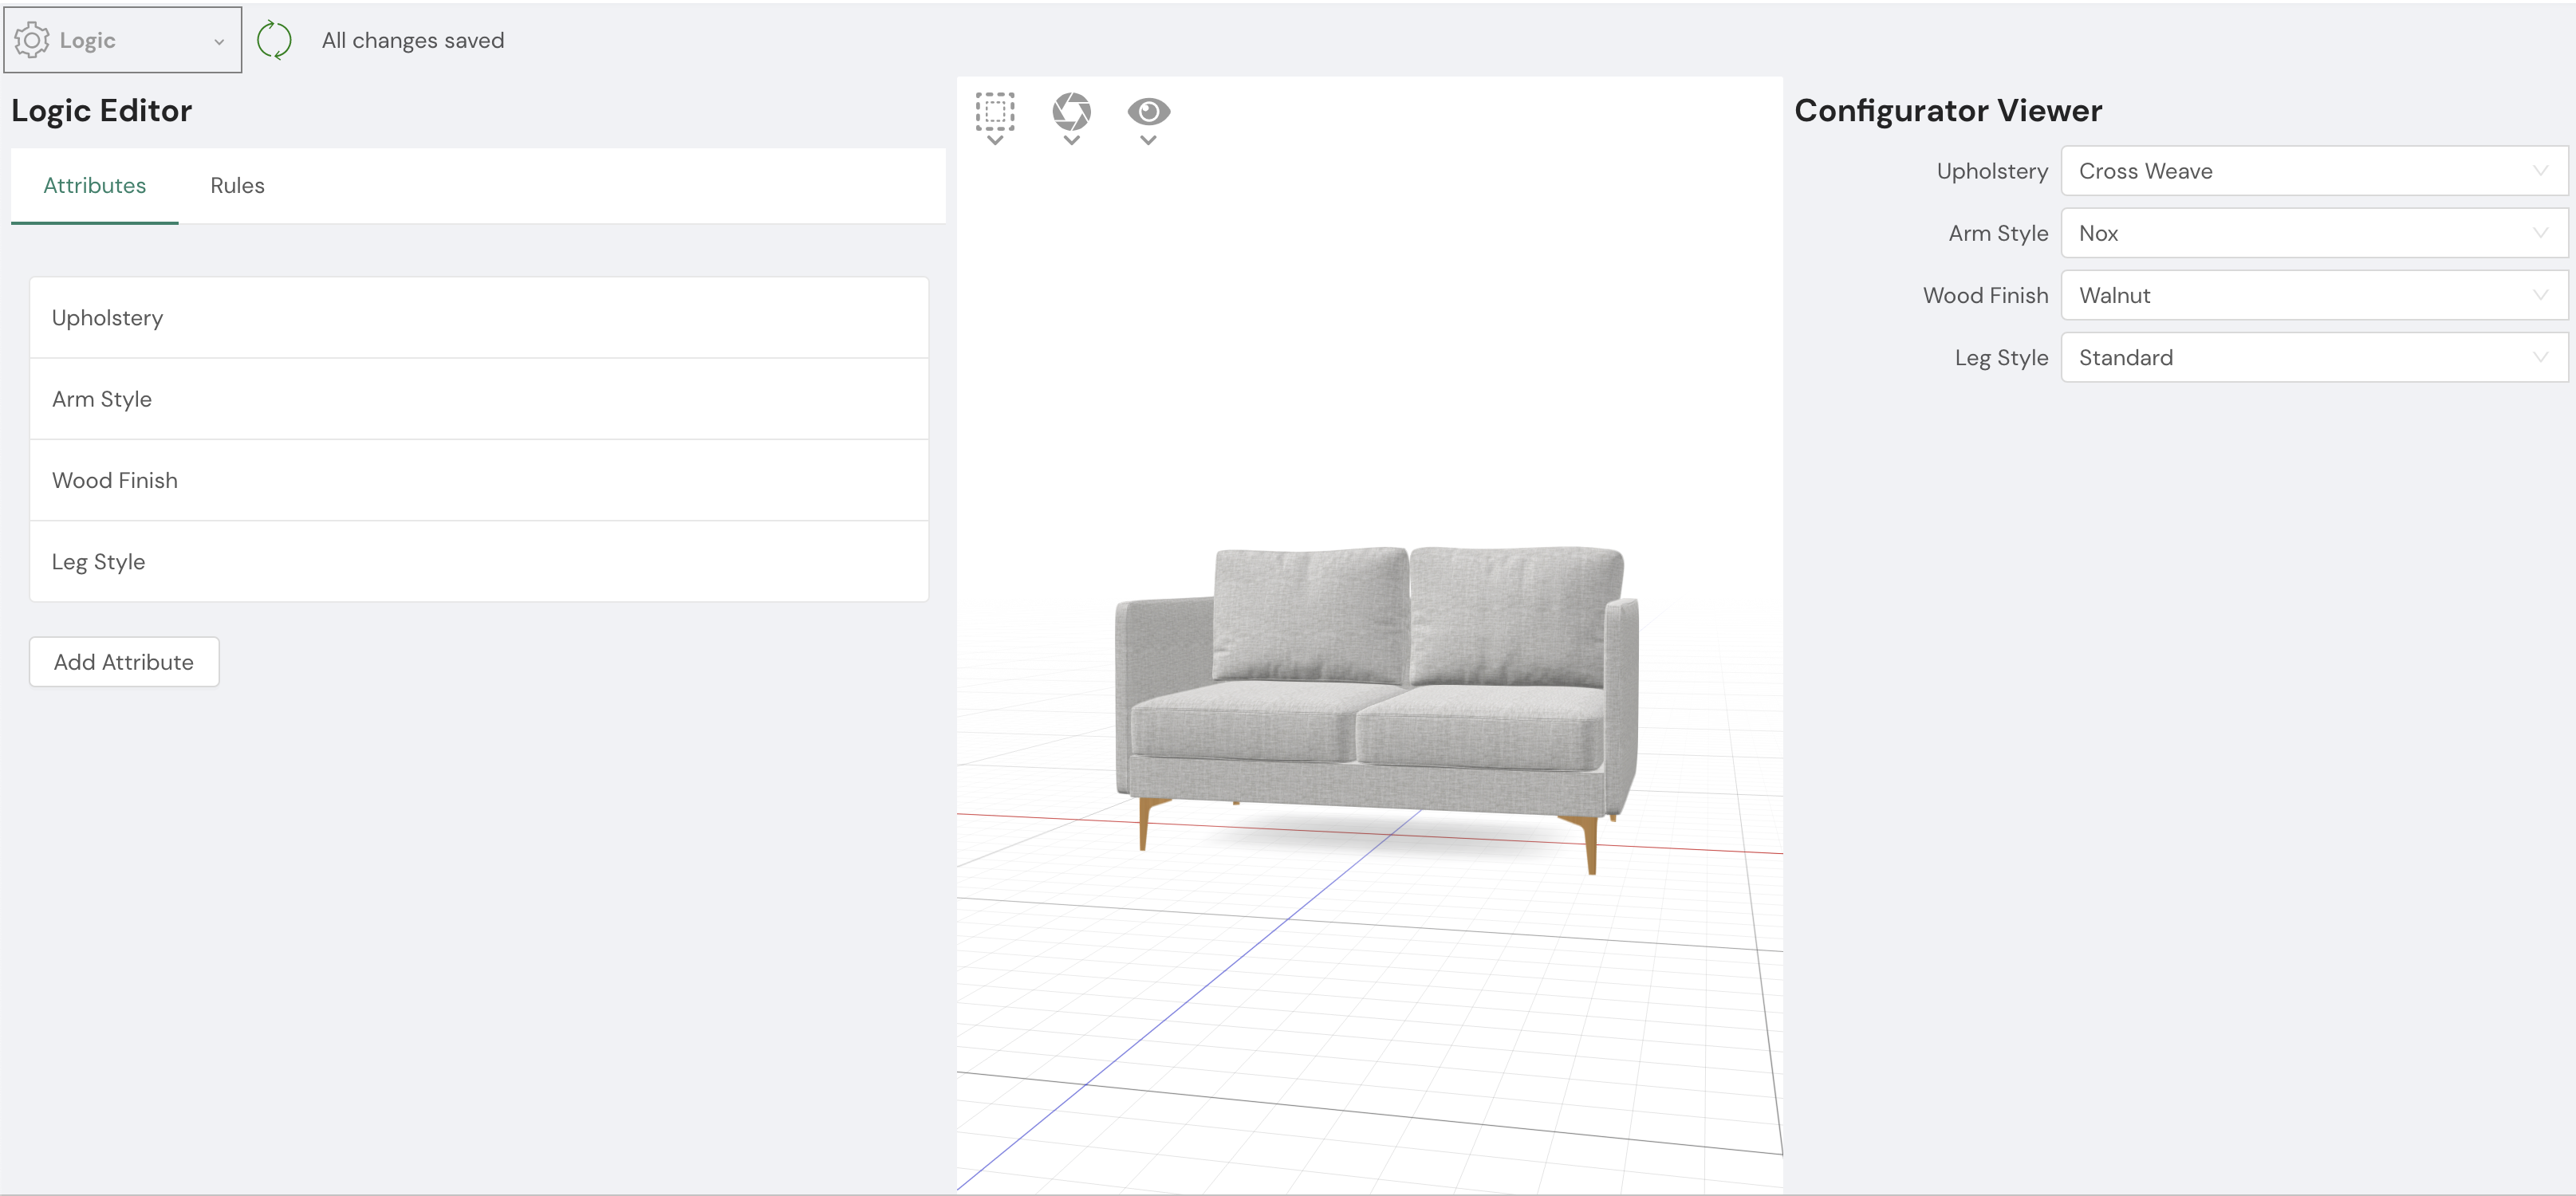
\includegraphics[width=14cm]{images/analysis_threekit-editor.png}
\captionsource{Threekit's Platform's editor}{Threekit Platform Documentation \cite{ThreeKitPlatformDocumentation}}
\label{fig:threekit-editor}
\end{figure}

\begin{figure}
\centering
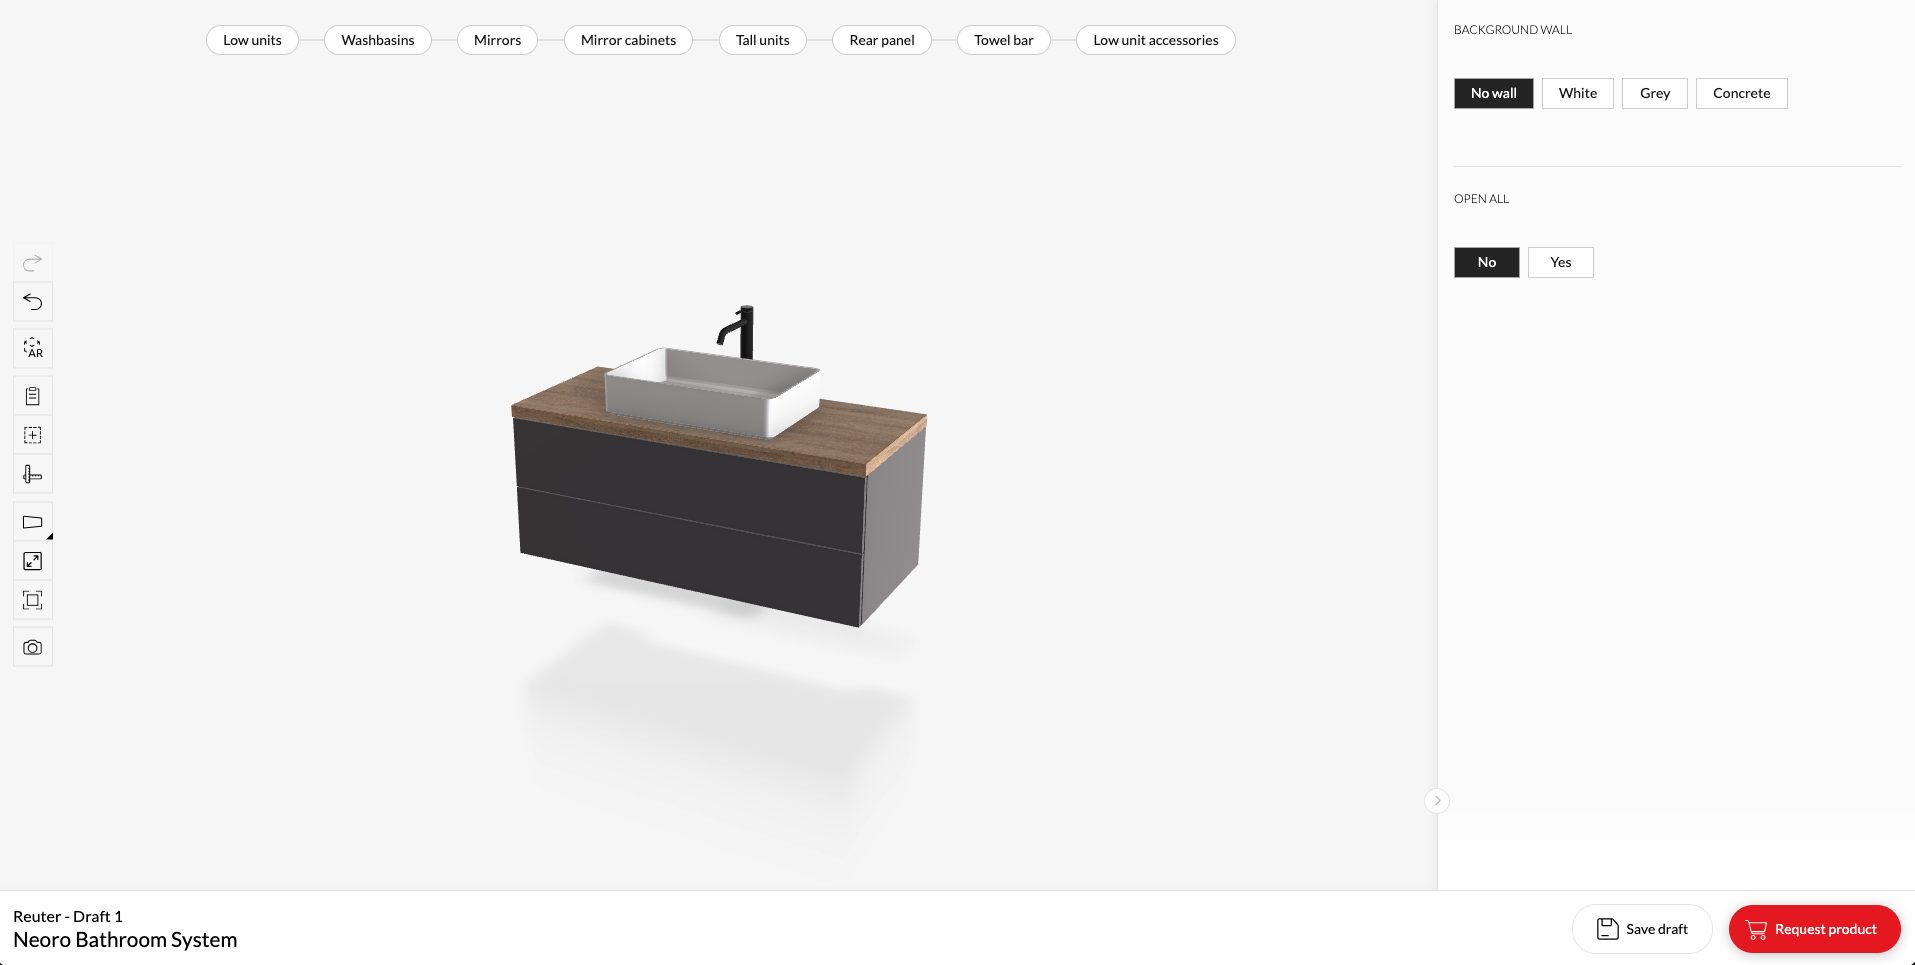
\includegraphics[width=14cm]{images/analysis_roomle.png}
\captionsource{Screenshot of Roomle's Rubens example}{Roomle Demos \cite{RoomleFullLogic}}
\label{fig:roomle}
\end{figure} % include `appendix.tex' from `text/' subdirectory
\chapter{Additional Code Listings} \label{appendix-b}

\begin{listing}
\begin{minted}{typescript}
const renderer = new THREE.WebGLRenderer();
renderer.setSize(window.innerWidth, window.innerHeight);
document.body.appendChild(renderer.domElement);

const scene = new THREE.Scene();

const geometry = new THREE.BoxGeometry(5, 5, 5);
const material = new THREE.MeshBasicMaterial({color: 0xff0000});
const mesh = new THREE.Mesh(geometry, material);
scene.add(mesh);

const camera = new THREE.PerspectiveCamera(
  75,
  window.innerWidth / window.innerHeight,
  0.1,
  1000
);
camera.position.set(10, 10, 10);
camera.lookAt(mesh.position);

renderer.render(scene, camera);
\end{minted}
\caption{Creating and displaying a 3D red cube with Three.js}
\label{listing:threejs}
\end{listing}

\begin{listing}
\begin{minted}{text}
const Component = () => {
    return (
        <Canvas camera={{position: [10, 10, 10]}}>
            <mesh>
                <meshBasicMaterial color="red" />
                <boxGeometry args={[5, 5, 5]} />
            </mesh>
        </Canvas>
    )
}
\end{minted}
\caption{Creating a 3D red cube as a React component with R3F}
\label{lisiting:r3f}
\end{listing}

\begin{listing}
\begin{minted}{typescript}
import { z } from 'zod';

const customSchema = z.number();

type CustomType = z.infer<typeof customSchema>;
\end{minted}
\captionsource{Conversion from Zod schema to TypeScript type}{Adapted from~\cite{Wycliffe2023}}
\label{listing:zod}
\end{listing}

\backmatter % do not remove this command

\todo{Add carrier (online) and dates to websites}
\printbibliography % print out the BibLaTeX-generated bibliography list

\chapter{Concents of the attachment}
% Concents of the attachment

	\dirtree{%
		.1 readme.txt\DTcomment{stručný popis obsahu média}.
		.1 exe\DTcomment{adresář se spustitelnou formou implementace}.
		.1 src.
		.2 impl\DTcomment{zdrojové kódy implementace}.
		.2 thesis\DTcomment{zdrojová forma práce ve formátu \LaTeX{}}.
		.1 text\DTcomment{text práce}.
		.2 thesis.pdf\DTcomment{text práce ve formátu PDF}.
	}
 % include `medium.tex' from `text/' subdirectory

\end{document}
